\documentclass[a4paper]{book}
\usepackage{makeidx}
\usepackage{natbib}
\usepackage{graphicx}
\usepackage{multicol}
\usepackage{float}
\usepackage{listings}
\usepackage{color}
\usepackage{ifthen}
\usepackage[table]{xcolor}
\usepackage{textcomp}
\usepackage{alltt}
\usepackage{ifpdf}
\ifpdf
\usepackage[pdftex,
            pagebackref=true,
            colorlinks=true,
            linkcolor=blue,
            unicode
           ]{hyperref}
\else
\usepackage[ps2pdf,
            pagebackref=true,
            colorlinks=true,
            linkcolor=blue,
            unicode
           ]{hyperref}
\usepackage{pspicture}
\fi
\usepackage[utf8]{inputenc}
\usepackage{mathptmx}
\usepackage[scaled=.90]{helvet}
\usepackage{courier}
\usepackage{sectsty}
\usepackage[titles]{tocloft}
\usepackage{doxygen}
\lstset{language=C++,inputencoding=utf8,basicstyle=\footnotesize,breaklines=true,breakatwhitespace=true,tabsize=8,numbers=left }
\makeindex
\setcounter{tocdepth}{3}
\renewcommand{\footrulewidth}{0.4pt}
\renewcommand{\familydefault}{\sfdefault}
\hfuzz=15pt
\setlength{\emergencystretch}{15pt}
\hbadness=750
\tolerance=750
\begin{document}
\hypersetup{pageanchor=false,citecolor=blue}
\begin{titlepage}
\vspace*{7cm}
\begin{center}
{\Large \-C\-V\-X\-\_\-\-Pose \\[1ex]\large 1.\-0 }\\
\vspace*{1cm}
{\large \-Generated by Doxygen 1.7.6.1}\\
\vspace*{0.5cm}
{\small Mon Jul 28 2014 12:03:21}\\
\end{center}
\end{titlepage}
\clearemptydoublepage
\pagenumbering{roman}
\tableofcontents
\clearemptydoublepage
\pagenumbering{arabic}
\hypersetup{pageanchor=true,citecolor=blue}
\chapter{\-Class \-Index}
\section{\-Class \-Hierarchy}
\-This inheritance list is sorted roughly, but not completely, alphabetically\-:\begin{DoxyCompactList}
\item \contentsline{section}{\-I\-C\-P}{\pageref{classICP}}{}
\item \contentsline{section}{\-Pose\-Estimate}{\pageref{classPoseEstimate}}{}
\begin{DoxyCompactList}
\item \contentsline{section}{\-Solve\-Pose\-Analytic}{\pageref{classSolvePoseAnalytic}}{}
\item \contentsline{section}{\-Solve\-Pose\-C\-V\-X}{\pageref{classSolvePoseCVX}}{}
\end{DoxyCompactList}
\item \contentsline{section}{\-Solver\-Settings}{\pageref{structSolverSettings}}{}
\end{DoxyCompactList}

\chapter{\-Class \-Index}
\section{\-Class \-List}
\-Here are the classes, structs, unions and interfaces with brief descriptions\-:\begin{DoxyCompactList}
\item\contentsline{section}{\hyperlink{classICP}{\-I\-C\-P} \\*\-Iterative \-Closest \-Point }{\pageref{classICP}}{}
\item\contentsline{section}{\hyperlink{classPoseEstimate}{\-Pose\-Estimate} \\*\-Class for performing pose estimation }{\pageref{classPoseEstimate}}{}
\item\contentsline{section}{\hyperlink{classSolvePoseAnalytic}{\-Solve\-Pose\-Analytic} \\*\-Pose estimation using analytic solutions to optimization problems over the convex hull of \-S\-O(3) }{\pageref{classSolvePoseAnalytic}}{}
\item\contentsline{section}{\hyperlink{classSolvePoseCVX}{\-Solve\-Pose\-C\-V\-X} \\*\-Pose estimation using the convex hull of \-S\-O(3) via a semidefinite program }{\pageref{classSolvePoseCVX}}{}
\item\contentsline{section}{\hyperlink{structSolverSettings}{\-Solver\-Settings} }{\pageref{structSolverSettings}}{}
\end{DoxyCompactList}

\chapter{\-File \-Index}
\section{\-File \-List}
\-Here is a list of all files with brief descriptions\-:\begin{DoxyCompactList}
\item\contentsline{section}{\-Cvx\-\_\-\-Pose/examples/\hyperlink{bunny_8cpp}{bunny.\-cpp} }{\pageref{bunny_8cpp}}{}
\item\contentsline{section}{\-Cvx\-\_\-\-Pose/src/\hyperlink{common_8h}{common.\-h} }{\pageref{common_8h}}{}
\item\contentsline{section}{\-Cvx\-\_\-\-Pose/src/\hyperlink{ICP_8cpp}{\-I\-C\-P.\-cpp} }{\pageref{ICP_8cpp}}{}
\item\contentsline{section}{\-Cvx\-\_\-\-Pose/src/\hyperlink{ICP_8h}{\-I\-C\-P.\-h} }{\pageref{ICP_8h}}{}
\item\contentsline{section}{\-Cvx\-\_\-\-Pose/src/\hyperlink{PoseEstimate_8cpp}{\-Pose\-Estimate.\-cpp} }{\pageref{PoseEstimate_8cpp}}{}
\item\contentsline{section}{\-Cvx\-\_\-\-Pose/src/\hyperlink{PoseEstimate_8h}{\-Pose\-Estimate.\-h} }{\pageref{PoseEstimate_8h}}{}
\item\contentsline{section}{\-Cvx\-\_\-\-Pose/src/\hyperlink{SolvePoseAnalytic_8cpp}{\-Solve\-Pose\-Analytic.\-cpp} }{\pageref{SolvePoseAnalytic_8cpp}}{}
\item\contentsline{section}{\-Cvx\-\_\-\-Pose/src/\hyperlink{SolvePoseAnalytic_8h}{\-Solve\-Pose\-Analytic.\-h} }{\pageref{SolvePoseAnalytic_8h}}{}
\item\contentsline{section}{\-Cvx\-\_\-\-Pose/src/\hyperlink{SolvePoseCVX_8cpp}{\-Solve\-Pose\-C\-V\-X.\-cpp} }{\pageref{SolvePoseCVX_8cpp}}{}
\item\contentsline{section}{\-Cvx\-\_\-\-Pose/src/\hyperlink{SolvePoseCVX_8h}{\-Solve\-Pose\-C\-V\-X.\-h} }{\pageref{SolvePoseCVX_8h}}{}
\end{DoxyCompactList}

\chapter{\-Class \-Documentation}
\hypertarget{classICP}{\section{\-I\-C\-P \-Class \-Reference}
\label{classICP}\index{\-I\-C\-P@{\-I\-C\-P}}
}


\-Iterative \-Closest \-Point.  




{\ttfamily \#include $<$\-I\-C\-P.\-h$>$}

\subsection*{\-Public \-Member \-Functions}
\begin{DoxyCompactItemize}
\item 
\hyperlink{classICP_a6a6f021c394b70387f0163239a74f94b}{\-I\-C\-P} ()
\begin{DoxyCompactList}\small\item\em \hyperlink{classICP}{\-I\-C\-P} default constructor. \end{DoxyCompactList}\item 
\hyperlink{classICP_a744eea059d43f0794b50d15ed056746a}{$\sim$\-I\-C\-P} ()
\begin{DoxyCompactList}\small\item\em \hyperlink{classICP}{\-I\-C\-P} destructor. \end{DoxyCompactList}\item 
void \hyperlink{classICP_a49b0a9fafd601c49f7cdd55edaa0f7a7}{set\-Solver} (\hyperlink{structSolverSettings}{\-Solver\-Settings} s)
\begin{DoxyCompactList}\small\item\em \-Set the solver settings. \end{DoxyCompactList}\item 
void \hyperlink{classICP_a7e02bf0f96bacf61fb7462c852be3c08}{set\-Model} (pcl\-::\-Point\-Cloud$<$ \hyperlink{common_8h_abd10555a534258e2739a38c928ef5db1}{\-Point\-T} $>$\-::\-Ptr m)
\begin{DoxyCompactList}\small\item\em \-Set the model which \hyperlink{classICP}{\-I\-C\-P} will use to estimate pose. \end{DoxyCompactList}\item 
void \hyperlink{classICP_a65d3a5293b19ec80f5f569abccd8b395}{set\-Observation} (pcl\-::\-Point\-Cloud$<$ \hyperlink{common_8h_abd10555a534258e2739a38c928ef5db1}{\-Point\-T} $>$\-::\-Ptr o)
\begin{DoxyCompactList}\small\item\em \-Set the observation which \hyperlink{classICP}{\-I\-C\-P} will try to match with its model. \end{DoxyCompactList}\item 
void \hyperlink{classICP_a8168f085dc9bf3916ea9b170f4a8b6f3}{est\-Pose} ()
\begin{DoxyCompactList}\small\item\em \-Perform the pose estimation iteration until convergence. \end{DoxyCompactList}\item 
void \hyperlink{classICP_a1dfd1ad0ea3c83ade91595cc3ecd24f2}{single\-Iteration} ()
\begin{DoxyCompactList}\small\item\em \-Single iteration of \hyperlink{classICP}{\-I\-C\-P}\-: correspondence then pose estimate. \end{DoxyCompactList}\item 
void \hyperlink{classICP_af9624105149162bf1c80b2e70cbcf135}{get\-Pose} (\-Eigen\-::\-Matrix3f \&rot, \-Eigen\-::\-Vector3f \&trans)
\begin{DoxyCompactList}\small\item\em \-Retrieve the estimated pose. \end{DoxyCompactList}\end{DoxyCompactItemize}
\subsection*{\-Protected \-Member \-Functions}
\begin{DoxyCompactItemize}
\item 
void \hyperlink{classICP_a5e20a89dfd2f5f95a61122d268375b72}{dbg} (std\-::string)
\begin{DoxyCompactList}\small\item\em \-Debug output. \end{DoxyCompactList}\end{DoxyCompactItemize}
\subsection*{\-Protected \-Attributes}
\begin{DoxyCompactItemize}
\item 
\-Eigen\-::\-Sparse\-Matrix$<$ float $>$ \hyperlink{classICP_aade0504cb0e1d5abcb2c2add2be606b1}{permutation}
\end{DoxyCompactItemize}
\subsection*{\-Private \-Attributes}
\begin{DoxyCompactItemize}
\item 
\hyperlink{structSolverSettings}{\-Solver\-Settings} \hyperlink{classICP_a7e3065919f63c9bdc0ff0677b5cf56d0}{settings}
\begin{DoxyCompactList}\small\item\em \-Stores the \hyperlink{classICP}{\-I\-C\-P} settings. \end{DoxyCompactList}\item 
\hyperlink{classPoseEstimate}{\-Pose\-Estimate} $\ast$ \hyperlink{classICP_a09c458b7e1daa98c6cc98177003794ce}{pose}
\begin{DoxyCompactList}\small\item\em \-Member for performing pose estimation. \end{DoxyCompactList}\item 
\-Eigen\-::\-Matrix3f \hyperlink{classICP_aee085ec283f657cb3980c529d48ba65b}{c\-\_\-\-R}
\begin{DoxyCompactList}\small\item\em \-Current rotation estimate. \end{DoxyCompactList}\item 
\-Eigen\-::\-Matrix3f \hyperlink{classICP_a07164ef6066cf0c9537881871cd56601}{i\-\_\-\-R}
\begin{DoxyCompactList}\small\item\em \-Initial rotation estimate supplied by user. \end{DoxyCompactList}\item 
\-Eigen\-::\-Vector3f \hyperlink{classICP_a55de298290d8e74617fdf19c153d55be}{c\-\_\-\-T}
\begin{DoxyCompactList}\small\item\em \-Current translation estimate. \end{DoxyCompactList}\item 
\-Eigen\-::\-Vector3f \hyperlink{classICP_a63b486fc85453b0f09c6020e1c6227f4}{i\-\_\-\-T}
\begin{DoxyCompactList}\small\item\em \-Initial translation estimate supplied by user. \end{DoxyCompactList}\item 
pcl\-::\-Point\-Cloud$<$ \hyperlink{common_8h_abd10555a534258e2739a38c928ef5db1}{\-Point\-T} $>$ \hyperlink{classICP_ae224713dd84e34bbef52a011046527af}{model}
\begin{DoxyCompactList}\small\item\em \-Internal model of the object whose pose is to be estimated. \end{DoxyCompactList}\item 
pcl\-::\-Point\-Cloud$<$ \hyperlink{common_8h_abd10555a534258e2739a38c928ef5db1}{\-Point\-T} $>$ \hyperlink{classICP_a92b2b3089759aad730cb92a0976aea1b}{observation}
\begin{DoxyCompactList}\small\item\em \-Internal copy of an object observation. \end{DoxyCompactList}\item 
pcl\-::registration\-::\-Correspondence\-Estimation\*
$<$ \hyperlink{common_8h_abd10555a534258e2739a38c928ef5db1}{\-Point\-T}, \hyperlink{common_8h_abd10555a534258e2739a38c928ef5db1}{\-Point\-T} $>$ \hyperlink{classICP_acf6194ebbf168e4a6059945980752849}{est}
\begin{DoxyCompactList}\small\item\em \-P\-C\-L class for estimating correspondence between model and observation points. \end{DoxyCompactList}\item 
int \hyperlink{classICP_a9b8cf5129a0cb5ad3fd05b261d514bb6}{num\-\_\-pts}
\begin{DoxyCompactList}\small\item\em \-Count of number of points in observation and model (which should be equal, for now). \end{DoxyCompactList}\item 
bool \hyperlink{classICP_a6e81d1444353ba66d59cd16d2dc74d7c}{debug}
\begin{DoxyCompactList}\small\item\em \-Setting for printing (or not) of debug messages. \end{DoxyCompactList}\end{DoxyCompactItemize}


\subsection{\-Detailed \-Description}
\-Iterative \-Closest \-Point. 

\-Class that manages the \hyperlink{classICP}{\-I\-C\-P} algorithm. \-It relies on a \-P\-C\-L class for performing correspondence, and a \hyperlink{classPoseEstimate}{\-Pose\-Estimate} instance for calculating the pose. \hyperlink{classICP}{\-I\-C\-P} iterates betweeen these two functions to find a pose and correspondence between a model and an observation of that model.

\begin{DoxyAuthor}{\-Author}
\-Matanya \-Horowitz 
\end{DoxyAuthor}
\begin{DoxyVersion}{\-Version}
1.\-0 
\end{DoxyVersion}
\begin{DoxyDate}{\-Date}
\-July 28, 2014 
\end{DoxyDate}


\subsection{\-Constructor \& \-Destructor \-Documentation}
\hypertarget{classICP_a6a6f021c394b70387f0163239a74f94b}{\index{\-I\-C\-P@{\-I\-C\-P}!\-I\-C\-P@{\-I\-C\-P}}
\index{\-I\-C\-P@{\-I\-C\-P}!ICP@{\-I\-C\-P}}
\subsubsection[{\-I\-C\-P}]{\setlength{\rightskip}{0pt plus 5cm}{\bf \-I\-C\-P\-::\-I\-C\-P} (
\begin{DoxyParamCaption}
{}
\end{DoxyParamCaption}
)}}\label{classICP_a6a6f021c394b70387f0163239a74f94b}


\hyperlink{classICP}{\-I\-C\-P} default constructor. 

\-Initializes pose and translation estimate to identity and the origin \hypertarget{classICP_a744eea059d43f0794b50d15ed056746a}{\index{\-I\-C\-P@{\-I\-C\-P}!$\sim$\-I\-C\-P@{$\sim$\-I\-C\-P}}
\index{$\sim$\-I\-C\-P@{$\sim$\-I\-C\-P}!ICP@{\-I\-C\-P}}
\subsubsection[{$\sim$\-I\-C\-P}]{\setlength{\rightskip}{0pt plus 5cm}{\bf \-I\-C\-P\-::$\sim$\-I\-C\-P} (
\begin{DoxyParamCaption}
{}
\end{DoxyParamCaption}
)}}\label{classICP_a744eea059d43f0794b50d15ed056746a}


\hyperlink{classICP}{\-I\-C\-P} destructor. 

\mbox{[}\-Todo\mbox{]} \-Currently, this is unimplemented and may be leaking memory. 

\subsection{\-Member \-Function \-Documentation}
\hypertarget{classICP_a5e20a89dfd2f5f95a61122d268375b72}{\index{\-I\-C\-P@{\-I\-C\-P}!dbg@{dbg}}
\index{dbg@{dbg}!ICP@{\-I\-C\-P}}
\subsubsection[{dbg}]{\setlength{\rightskip}{0pt plus 5cm}void {\bf \-I\-C\-P\-::dbg} (
\begin{DoxyParamCaption}
\item[{std\-::string}]{msg}
\end{DoxyParamCaption}
)\hspace{0.3cm}{\ttfamily  \mbox{[}protected\mbox{]}}}}\label{classICP_a5e20a89dfd2f5f95a61122d268375b72}


\-Debug output. 

\-Very rough for now, simply prints or not depending on the debug flag. 
\begin{DoxyParams}[1]{\-Parameters}
\mbox{\tt in}  & {\em msg} & \-The debug message \\
\hline
\end{DoxyParams}
\hypertarget{classICP_a8168f085dc9bf3916ea9b170f4a8b6f3}{\index{\-I\-C\-P@{\-I\-C\-P}!est\-Pose@{est\-Pose}}
\index{est\-Pose@{est\-Pose}!ICP@{\-I\-C\-P}}
\subsubsection[{est\-Pose}]{\setlength{\rightskip}{0pt plus 5cm}void {\bf \-I\-C\-P\-::est\-Pose} (
\begin{DoxyParamCaption}
{}
\end{DoxyParamCaption}
)}}\label{classICP_a8168f085dc9bf3916ea9b170f4a8b6f3}


\-Perform the pose estimation iteration until convergence. 

\mbox{[}\-Todo\mbox{]} \-In the future, a coarse alignment will first be performed with a down sampled model, or using depth features.

\mbox{[}\-Todo\mbox{]} \-In the future, there will be an option to begin with multiple pose initial conditions \hypertarget{classICP_af9624105149162bf1c80b2e70cbcf135}{\index{\-I\-C\-P@{\-I\-C\-P}!get\-Pose@{get\-Pose}}
\index{get\-Pose@{get\-Pose}!ICP@{\-I\-C\-P}}
\subsubsection[{get\-Pose}]{\setlength{\rightskip}{0pt plus 5cm}void {\bf \-I\-C\-P\-::get\-Pose} (
\begin{DoxyParamCaption}
\item[{\-Eigen\-::\-Matrix3f \&}]{rot, }
\item[{\-Eigen\-::\-Vector3f \&}]{trans}
\end{DoxyParamCaption}
)}}\label{classICP_af9624105149162bf1c80b2e70cbcf135}


\-Retrieve the estimated pose. 


\begin{DoxyParams}[1]{\-Parameters}
\mbox{\tt out}  & {\em rot} & \-The rotation matrix \\
\hline
\mbox{\tt out}  & {\em trans} & \-The translation vector \\
\hline
\end{DoxyParams}
\hypertarget{classICP_a7e02bf0f96bacf61fb7462c852be3c08}{\index{\-I\-C\-P@{\-I\-C\-P}!set\-Model@{set\-Model}}
\index{set\-Model@{set\-Model}!ICP@{\-I\-C\-P}}
\subsubsection[{set\-Model}]{\setlength{\rightskip}{0pt plus 5cm}void {\bf \-I\-C\-P\-::set\-Model} (
\begin{DoxyParamCaption}
\item[{pcl\-::\-Point\-Cloud$<$ {\bf \-Point\-T} $>$\-::\-Ptr}]{m}
\end{DoxyParamCaption}
)}}\label{classICP_a7e02bf0f96bacf61fb7462c852be3c08}


\-Set the model which \hyperlink{classICP}{\-I\-C\-P} will use to estimate pose. 


\begin{DoxyParams}[1]{\-Parameters}
\mbox{\tt in}  & {\em m} & \-P\-C\-L pointer to the model. \\
\hline
\end{DoxyParams}
\hypertarget{classICP_a65d3a5293b19ec80f5f569abccd8b395}{\index{\-I\-C\-P@{\-I\-C\-P}!set\-Observation@{set\-Observation}}
\index{set\-Observation@{set\-Observation}!ICP@{\-I\-C\-P}}
\subsubsection[{set\-Observation}]{\setlength{\rightskip}{0pt plus 5cm}void {\bf \-I\-C\-P\-::set\-Observation} (
\begin{DoxyParamCaption}
\item[{pcl\-::\-Point\-Cloud$<$ {\bf \-Point\-T} $>$\-::\-Ptr}]{o}
\end{DoxyParamCaption}
)}}\label{classICP_a65d3a5293b19ec80f5f569abccd8b395}


\-Set the observation which \hyperlink{classICP}{\-I\-C\-P} will try to match with its model. 

\hypertarget{classICP_a49b0a9fafd601c49f7cdd55edaa0f7a7}{\index{\-I\-C\-P@{\-I\-C\-P}!set\-Solver@{set\-Solver}}
\index{set\-Solver@{set\-Solver}!ICP@{\-I\-C\-P}}
\subsubsection[{set\-Solver}]{\setlength{\rightskip}{0pt plus 5cm}void {\bf \-I\-C\-P\-::set\-Solver} (
\begin{DoxyParamCaption}
\item[{{\bf \-Solver\-Settings}}]{s}
\end{DoxyParamCaption}
)}}\label{classICP_a49b0a9fafd601c49f7cdd55edaa0f7a7}


\-Set the solver settings. 


\begin{DoxyParams}[1]{\-Parameters}
\mbox{\tt in}  & {\em s} & \-Complete specification of problem settings. \\
\hline
\end{DoxyParams}
\hypertarget{classICP_a1dfd1ad0ea3c83ade91595cc3ecd24f2}{\index{\-I\-C\-P@{\-I\-C\-P}!single\-Iteration@{single\-Iteration}}
\index{single\-Iteration@{single\-Iteration}!ICP@{\-I\-C\-P}}
\subsubsection[{single\-Iteration}]{\setlength{\rightskip}{0pt plus 5cm}void {\bf \-I\-C\-P\-::single\-Iteration} (
\begin{DoxyParamCaption}
{}
\end{DoxyParamCaption}
)}}\label{classICP_a1dfd1ad0ea3c83ade91595cc3ecd24f2}


\-Single iteration of \hyperlink{classICP}{\-I\-C\-P}\-: correspondence then pose estimate. 



\subsection{\-Member \-Data \-Documentation}
\hypertarget{classICP_aee085ec283f657cb3980c529d48ba65b}{\index{\-I\-C\-P@{\-I\-C\-P}!c\-\_\-\-R@{c\-\_\-\-R}}
\index{c\-\_\-\-R@{c\-\_\-\-R}!ICP@{\-I\-C\-P}}
\subsubsection[{c\-\_\-\-R}]{\setlength{\rightskip}{0pt plus 5cm}\-Eigen\-::\-Matrix3f {\bf \-I\-C\-P\-::c\-\_\-\-R}\hspace{0.3cm}{\ttfamily  \mbox{[}private\mbox{]}}}}\label{classICP_aee085ec283f657cb3980c529d48ba65b}


\-Current rotation estimate. 

\hypertarget{classICP_a55de298290d8e74617fdf19c153d55be}{\index{\-I\-C\-P@{\-I\-C\-P}!c\-\_\-\-T@{c\-\_\-\-T}}
\index{c\-\_\-\-T@{c\-\_\-\-T}!ICP@{\-I\-C\-P}}
\subsubsection[{c\-\_\-\-T}]{\setlength{\rightskip}{0pt plus 5cm}\-Eigen\-::\-Vector3f {\bf \-I\-C\-P\-::c\-\_\-\-T}\hspace{0.3cm}{\ttfamily  \mbox{[}private\mbox{]}}}}\label{classICP_a55de298290d8e74617fdf19c153d55be}


\-Current translation estimate. 

\hypertarget{classICP_a6e81d1444353ba66d59cd16d2dc74d7c}{\index{\-I\-C\-P@{\-I\-C\-P}!debug@{debug}}
\index{debug@{debug}!ICP@{\-I\-C\-P}}
\subsubsection[{debug}]{\setlength{\rightskip}{0pt plus 5cm}bool {\bf \-I\-C\-P\-::debug}\hspace{0.3cm}{\ttfamily  \mbox{[}private\mbox{]}}}}\label{classICP_a6e81d1444353ba66d59cd16d2dc74d7c}


\-Setting for printing (or not) of debug messages. 

\hypertarget{classICP_acf6194ebbf168e4a6059945980752849}{\index{\-I\-C\-P@{\-I\-C\-P}!est@{est}}
\index{est@{est}!ICP@{\-I\-C\-P}}
\subsubsection[{est}]{\setlength{\rightskip}{0pt plus 5cm}pcl\-::registration\-::\-Correspondence\-Estimation$<${\bf \-Point\-T}, {\bf \-Point\-T}$>$ {\bf \-I\-C\-P\-::est}\hspace{0.3cm}{\ttfamily  \mbox{[}private\mbox{]}}}}\label{classICP_acf6194ebbf168e4a6059945980752849}


\-P\-C\-L class for estimating correspondence between model and observation points. 

\hypertarget{classICP_a07164ef6066cf0c9537881871cd56601}{\index{\-I\-C\-P@{\-I\-C\-P}!i\-\_\-\-R@{i\-\_\-\-R}}
\index{i\-\_\-\-R@{i\-\_\-\-R}!ICP@{\-I\-C\-P}}
\subsubsection[{i\-\_\-\-R}]{\setlength{\rightskip}{0pt plus 5cm}\-Eigen\-::\-Matrix3f {\bf \-I\-C\-P\-::i\-\_\-\-R}\hspace{0.3cm}{\ttfamily  \mbox{[}private\mbox{]}}}}\label{classICP_a07164ef6066cf0c9537881871cd56601}


\-Initial rotation estimate supplied by user. 

\hypertarget{classICP_a63b486fc85453b0f09c6020e1c6227f4}{\index{\-I\-C\-P@{\-I\-C\-P}!i\-\_\-\-T@{i\-\_\-\-T}}
\index{i\-\_\-\-T@{i\-\_\-\-T}!ICP@{\-I\-C\-P}}
\subsubsection[{i\-\_\-\-T}]{\setlength{\rightskip}{0pt plus 5cm}\-Eigen\-::\-Vector3f {\bf \-I\-C\-P\-::i\-\_\-\-T}\hspace{0.3cm}{\ttfamily  \mbox{[}private\mbox{]}}}}\label{classICP_a63b486fc85453b0f09c6020e1c6227f4}


\-Initial translation estimate supplied by user. 

\hypertarget{classICP_ae224713dd84e34bbef52a011046527af}{\index{\-I\-C\-P@{\-I\-C\-P}!model@{model}}
\index{model@{model}!ICP@{\-I\-C\-P}}
\subsubsection[{model}]{\setlength{\rightskip}{0pt plus 5cm}pcl\-::\-Point\-Cloud$<${\bf \-Point\-T}$>$ {\bf \-I\-C\-P\-::model}\hspace{0.3cm}{\ttfamily  \mbox{[}private\mbox{]}}}}\label{classICP_ae224713dd84e34bbef52a011046527af}


\-Internal model of the object whose pose is to be estimated. 

\hypertarget{classICP_a9b8cf5129a0cb5ad3fd05b261d514bb6}{\index{\-I\-C\-P@{\-I\-C\-P}!num\-\_\-pts@{num\-\_\-pts}}
\index{num\-\_\-pts@{num\-\_\-pts}!ICP@{\-I\-C\-P}}
\subsubsection[{num\-\_\-pts}]{\setlength{\rightskip}{0pt plus 5cm}int {\bf \-I\-C\-P\-::num\-\_\-pts}\hspace{0.3cm}{\ttfamily  \mbox{[}private\mbox{]}}}}\label{classICP_a9b8cf5129a0cb5ad3fd05b261d514bb6}


\-Count of number of points in observation and model (which should be equal, for now). 

\hypertarget{classICP_a92b2b3089759aad730cb92a0976aea1b}{\index{\-I\-C\-P@{\-I\-C\-P}!observation@{observation}}
\index{observation@{observation}!ICP@{\-I\-C\-P}}
\subsubsection[{observation}]{\setlength{\rightskip}{0pt plus 5cm}pcl\-::\-Point\-Cloud$<${\bf \-Point\-T}$>$ {\bf \-I\-C\-P\-::observation}\hspace{0.3cm}{\ttfamily  \mbox{[}private\mbox{]}}}}\label{classICP_a92b2b3089759aad730cb92a0976aea1b}


\-Internal copy of an object observation. 

\hypertarget{classICP_aade0504cb0e1d5abcb2c2add2be606b1}{\index{\-I\-C\-P@{\-I\-C\-P}!permutation@{permutation}}
\index{permutation@{permutation}!ICP@{\-I\-C\-P}}
\subsubsection[{permutation}]{\setlength{\rightskip}{0pt plus 5cm}\-Eigen\-::\-Sparse\-Matrix$<$float$>$ {\bf \-I\-C\-P\-::permutation}\hspace{0.3cm}{\ttfamily  \mbox{[}protected\mbox{]}}}}\label{classICP_aade0504cb0e1d5abcb2c2add2be606b1}
\hypertarget{classICP_a09c458b7e1daa98c6cc98177003794ce}{\index{\-I\-C\-P@{\-I\-C\-P}!pose@{pose}}
\index{pose@{pose}!ICP@{\-I\-C\-P}}
\subsubsection[{pose}]{\setlength{\rightskip}{0pt plus 5cm}{\bf \-Pose\-Estimate}$\ast$ {\bf \-I\-C\-P\-::pose}\hspace{0.3cm}{\ttfamily  \mbox{[}private\mbox{]}}}}\label{classICP_a09c458b7e1daa98c6cc98177003794ce}


\-Member for performing pose estimation. 

\hypertarget{classICP_a7e3065919f63c9bdc0ff0677b5cf56d0}{\index{\-I\-C\-P@{\-I\-C\-P}!settings@{settings}}
\index{settings@{settings}!ICP@{\-I\-C\-P}}
\subsubsection[{settings}]{\setlength{\rightskip}{0pt plus 5cm}{\bf \-Solver\-Settings} {\bf \-I\-C\-P\-::settings}\hspace{0.3cm}{\ttfamily  \mbox{[}private\mbox{]}}}}\label{classICP_a7e3065919f63c9bdc0ff0677b5cf56d0}


\-Stores the \hyperlink{classICP}{\-I\-C\-P} settings. 

\-Shared with \hyperlink{classPoseEstimate}{\-Pose\-Estimate}. 

\-The documentation for this class was generated from the following files\-:\begin{DoxyCompactItemize}
\item 
\-Cvx\-\_\-\-Pose/src/\hyperlink{ICP_8h}{\-I\-C\-P.\-h}\item 
\-Cvx\-\_\-\-Pose/src/\hyperlink{ICP_8cpp}{\-I\-C\-P.\-cpp}\end{DoxyCompactItemize}

\hypertarget{classPoseEstimate}{\section{\-Pose\-Estimate \-Class \-Reference}
\label{classPoseEstimate}\index{\-Pose\-Estimate@{\-Pose\-Estimate}}
}


{\ttfamily \#include $<$\-Pose\-Estimate.\-h$>$}

\-Inheritance diagram for \-Pose\-Estimate\-:\begin{figure}[H]
\begin{center}
\leavevmode
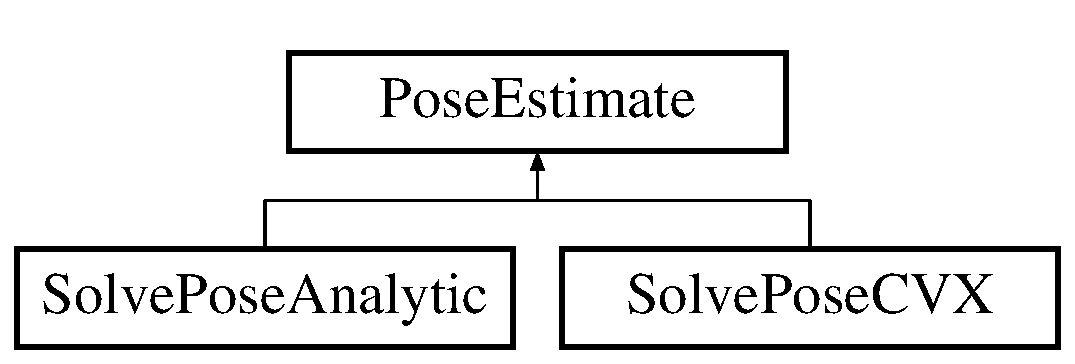
\includegraphics[height=2.000000cm]{classPoseEstimate}
\end{center}
\end{figure}
\subsection*{\-Public \-Member \-Functions}
\begin{DoxyCompactItemize}
\item 
\hyperlink{classPoseEstimate_ac3e3718fe27dccb3be0760d6bcdc18c6}{\-Pose\-Estimate} ()
\item 
\hyperlink{classPoseEstimate_ac024bd041a98d233647f106e6878d986}{$\sim$\-Pose\-Estimate} ()
\item 
virtual void \hyperlink{classPoseEstimate_a6fdf8eec3cadac69bcf8181c89d82903}{estimate\-Pose} ()=0
\item 
virtual void \hyperlink{classPoseEstimate_a4c420a20ba20719f7c19b8bbec79b6d9}{set\-Model} (pcl\-::\-Point\-Cloud$<$ \hyperlink{common_8h_abd10555a534258e2739a38c928ef5db1}{\-Point\-T} $>$\-::\-Ptr \hyperlink{classPoseEstimate_aca9217cfe0d272f172f65adfc31764f1}{model})
\item 
void \hyperlink{classPoseEstimate_ae884275e741789db776be52f373f387f}{set\-Observation} (pcl\-::\-Point\-Cloud$<$ \hyperlink{common_8h_abd10555a534258e2739a38c928ef5db1}{\-Point\-T} $>$\-::\-Ptr \hyperlink{classPoseEstimate_a75beb14fe9fd10fc8a80eff84f348c1c}{obs})
\item 
void \hyperlink{classPoseEstimate_a9daadf84954e07d295c2286172f01904}{permute\-Data} (\-Eigen\-::\-Sparse\-Matrix$<$ float $>$ \&\-P)
\item 
void \hyperlink{classPoseEstimate_af36ed6ccd1839eedff0f51f0bdaa23c7}{set\-Initial\-Pose} (\-Eigen\-::\-Matrix3f \&rot, \-Eigen\-::\-Vector3f \&trans)
\item 
void \hyperlink{classPoseEstimate_aa52680b9860a5a33201dfdd888e34c5a}{get\-Pose} (\-Eigen\-::\-Matrix3f \&rot, \-Eigen\-::\-Vector3f \&trans)
\item 
void \hyperlink{classPoseEstimate_a82d9fbf262d32338a9275f9cedee3f6c}{set\-Cores} (int num)
\item 
void \hyperlink{classPoseEstimate_a97197a2b7b19b8a975984841feaab1dc}{dbg} (std\-::string)
\item 
void \hyperlink{classPoseEstimate_a32bcf3736214b6635f9da6ad6be5f0ce}{calculate\-Centroid} (\hyperlink{common_8h_a4ec92c19d079ab17709ca464cfb8e5bd}{\-D\-Mat} \&data, \-Eigen\-::\-Vector3f \&center)
\item 
float \hyperlink{classPoseEstimate_ae195b53478db98ca075a6f0359ea422c}{calculate\-Residual} ()
\end{DoxyCompactItemize}
\subsection*{\-Protected \-Attributes}
\begin{DoxyCompactItemize}
\item 
\hyperlink{common_8h_a4ec92c19d079ab17709ca464cfb8e5bd}{\-D\-Mat} \hyperlink{classPoseEstimate_aca9217cfe0d272f172f65adfc31764f1}{model}
\item 
\hyperlink{common_8h_a4ec92c19d079ab17709ca464cfb8e5bd}{\-D\-Mat} \hyperlink{classPoseEstimate_a75beb14fe9fd10fc8a80eff84f348c1c}{obs}
\item 
\-Eigen\-::\-Matrix4f \hyperlink{classPoseEstimate_ad4827d1aca3b4730d6e8c0cf4e96deca}{\-A} \mbox{[}3\mbox{]}\mbox{[}3\mbox{]}
\item 
\-Eigen\-::\-Matrix3f \hyperlink{classPoseEstimate_a45910f753f4c92260252d965af504cc8}{\-R}
\item 
\-Eigen\-::\-Matrix3f \hyperlink{classPoseEstimate_ac6b2c23e4121d00a14d4a8245cad86ab}{i\-\_\-\-R}
\item 
\-Eigen\-::\-Vector3f \hyperlink{classPoseEstimate_a31a1a39ab75efc08a00ddc8f8f75b60b}{\-T}
\item 
\-Eigen\-::\-Vector3f \hyperlink{classPoseEstimate_a0fa85e3f7cd2b447df9985519a28c0d7}{i\-\_\-\-T}
\item 
int \hyperlink{classPoseEstimate_a9b1cbebd4de554e6c0b4607a2a462a92}{cores}
\item 
bool \hyperlink{classPoseEstimate_a81f2cf4c423887225557200a6da5744e}{debug}
\item 
int \hyperlink{classPoseEstimate_a8bad9dfcf6b8ec9e3ba4f62498594524}{num\-\_\-pts}
\item 
\-Eigen\-::\-Vector3f \hyperlink{classPoseEstimate_acd4fefbc3f3fd794f51a8a338996b2ae}{model\-\_\-center}
\item 
\-Eigen\-::\-Vector3f \hyperlink{classPoseEstimate_a3431f3d795bc7e5ec3108c923cf4eb9f}{obs\-\_\-center}
\item 
\hyperlink{structSolverSettings}{\-Solver\-Settings} \hyperlink{classPoseEstimate_ae1d0b8586991b50d575afa6b8bae92da}{settings}
\end{DoxyCompactItemize}


\subsection{\-Constructor \& \-Destructor \-Documentation}
\hypertarget{classPoseEstimate_ac3e3718fe27dccb3be0760d6bcdc18c6}{\index{\-Pose\-Estimate@{\-Pose\-Estimate}!\-Pose\-Estimate@{\-Pose\-Estimate}}
\index{\-Pose\-Estimate@{\-Pose\-Estimate}!PoseEstimate@{\-Pose\-Estimate}}
\subsubsection[{\-Pose\-Estimate}]{\setlength{\rightskip}{0pt plus 5cm}{\bf \-Pose\-Estimate\-::\-Pose\-Estimate} (
\begin{DoxyParamCaption}
{}
\end{DoxyParamCaption}
)}}\label{classPoseEstimate_ac3e3718fe27dccb3be0760d6bcdc18c6}
\hypertarget{classPoseEstimate_ac024bd041a98d233647f106e6878d986}{\index{\-Pose\-Estimate@{\-Pose\-Estimate}!$\sim$\-Pose\-Estimate@{$\sim$\-Pose\-Estimate}}
\index{$\sim$\-Pose\-Estimate@{$\sim$\-Pose\-Estimate}!PoseEstimate@{\-Pose\-Estimate}}
\subsubsection[{$\sim$\-Pose\-Estimate}]{\setlength{\rightskip}{0pt plus 5cm}{\bf \-Pose\-Estimate\-::$\sim$\-Pose\-Estimate} (
\begin{DoxyParamCaption}
{}
\end{DoxyParamCaption}
)}}\label{classPoseEstimate_ac024bd041a98d233647f106e6878d986}


\subsection{\-Member \-Function \-Documentation}
\hypertarget{classPoseEstimate_a32bcf3736214b6635f9da6ad6be5f0ce}{\index{\-Pose\-Estimate@{\-Pose\-Estimate}!calculate\-Centroid@{calculate\-Centroid}}
\index{calculate\-Centroid@{calculate\-Centroid}!PoseEstimate@{\-Pose\-Estimate}}
\subsubsection[{calculate\-Centroid}]{\setlength{\rightskip}{0pt plus 5cm}void {\bf \-Pose\-Estimate\-::calculate\-Centroid} (
\begin{DoxyParamCaption}
\item[{{\bf \-D\-Mat} \&}]{data, }
\item[{\-Eigen\-::\-Vector3f \&}]{center}
\end{DoxyParamCaption}
)}}\label{classPoseEstimate_a32bcf3736214b6635f9da6ad6be5f0ce}
\hypertarget{classPoseEstimate_ae195b53478db98ca075a6f0359ea422c}{\index{\-Pose\-Estimate@{\-Pose\-Estimate}!calculate\-Residual@{calculate\-Residual}}
\index{calculate\-Residual@{calculate\-Residual}!PoseEstimate@{\-Pose\-Estimate}}
\subsubsection[{calculate\-Residual}]{\setlength{\rightskip}{0pt plus 5cm}float {\bf \-Pose\-Estimate\-::calculate\-Residual} (
\begin{DoxyParamCaption}
{}
\end{DoxyParamCaption}
)}}\label{classPoseEstimate_ae195b53478db98ca075a6f0359ea422c}
\hypertarget{classPoseEstimate_a97197a2b7b19b8a975984841feaab1dc}{\index{\-Pose\-Estimate@{\-Pose\-Estimate}!dbg@{dbg}}
\index{dbg@{dbg}!PoseEstimate@{\-Pose\-Estimate}}
\subsubsection[{dbg}]{\setlength{\rightskip}{0pt plus 5cm}void {\bf \-Pose\-Estimate\-::dbg} (
\begin{DoxyParamCaption}
\item[{std\-::string}]{msg}
\end{DoxyParamCaption}
)}}\label{classPoseEstimate_a97197a2b7b19b8a975984841feaab1dc}
\hypertarget{classPoseEstimate_a6fdf8eec3cadac69bcf8181c89d82903}{\index{\-Pose\-Estimate@{\-Pose\-Estimate}!estimate\-Pose@{estimate\-Pose}}
\index{estimate\-Pose@{estimate\-Pose}!PoseEstimate@{\-Pose\-Estimate}}
\subsubsection[{estimate\-Pose}]{\setlength{\rightskip}{0pt plus 5cm}virtual void {\bf \-Pose\-Estimate\-::estimate\-Pose} (
\begin{DoxyParamCaption}
{}
\end{DoxyParamCaption}
)\hspace{0.3cm}{\ttfamily  \mbox{[}pure virtual\mbox{]}}}}\label{classPoseEstimate_a6fdf8eec3cadac69bcf8181c89d82903}


\-Implemented in \hyperlink{classSolvePoseAnalytic_a0a3fd0af007d4a945c03f49f820badcf}{\-Solve\-Pose\-Analytic}, and \hyperlink{classSolvePoseCVX_a081c857ff6c1c9e6597d41fb08bb6f16}{\-Solve\-Pose\-C\-V\-X}.

\hypertarget{classPoseEstimate_aa52680b9860a5a33201dfdd888e34c5a}{\index{\-Pose\-Estimate@{\-Pose\-Estimate}!get\-Pose@{get\-Pose}}
\index{get\-Pose@{get\-Pose}!PoseEstimate@{\-Pose\-Estimate}}
\subsubsection[{get\-Pose}]{\setlength{\rightskip}{0pt plus 5cm}void {\bf \-Pose\-Estimate\-::get\-Pose} (
\begin{DoxyParamCaption}
\item[{\-Eigen\-::\-Matrix3f \&}]{rot, }
\item[{\-Eigen\-::\-Vector3f \&}]{trans}
\end{DoxyParamCaption}
)}}\label{classPoseEstimate_aa52680b9860a5a33201dfdd888e34c5a}
\hypertarget{classPoseEstimate_a9daadf84954e07d295c2286172f01904}{\index{\-Pose\-Estimate@{\-Pose\-Estimate}!permute\-Data@{permute\-Data}}
\index{permute\-Data@{permute\-Data}!PoseEstimate@{\-Pose\-Estimate}}
\subsubsection[{permute\-Data}]{\setlength{\rightskip}{0pt plus 5cm}void {\bf \-Pose\-Estimate\-::permute\-Data} (
\begin{DoxyParamCaption}
\item[{\-Eigen\-::\-Sparse\-Matrix$<$ float $>$ \&}]{\-P}
\end{DoxyParamCaption}
)}}\label{classPoseEstimate_a9daadf84954e07d295c2286172f01904}
\hypertarget{classPoseEstimate_a82d9fbf262d32338a9275f9cedee3f6c}{\index{\-Pose\-Estimate@{\-Pose\-Estimate}!set\-Cores@{set\-Cores}}
\index{set\-Cores@{set\-Cores}!PoseEstimate@{\-Pose\-Estimate}}
\subsubsection[{set\-Cores}]{\setlength{\rightskip}{0pt plus 5cm}void {\bf \-Pose\-Estimate\-::set\-Cores} (
\begin{DoxyParamCaption}
\item[{int}]{num}
\end{DoxyParamCaption}
)}}\label{classPoseEstimate_a82d9fbf262d32338a9275f9cedee3f6c}
\hypertarget{classPoseEstimate_af36ed6ccd1839eedff0f51f0bdaa23c7}{\index{\-Pose\-Estimate@{\-Pose\-Estimate}!set\-Initial\-Pose@{set\-Initial\-Pose}}
\index{set\-Initial\-Pose@{set\-Initial\-Pose}!PoseEstimate@{\-Pose\-Estimate}}
\subsubsection[{set\-Initial\-Pose}]{\setlength{\rightskip}{0pt plus 5cm}void {\bf \-Pose\-Estimate\-::set\-Initial\-Pose} (
\begin{DoxyParamCaption}
\item[{\-Eigen\-::\-Matrix3f \&}]{rot, }
\item[{\-Eigen\-::\-Vector3f \&}]{trans}
\end{DoxyParamCaption}
)}}\label{classPoseEstimate_af36ed6ccd1839eedff0f51f0bdaa23c7}
\hypertarget{classPoseEstimate_a4c420a20ba20719f7c19b8bbec79b6d9}{\index{\-Pose\-Estimate@{\-Pose\-Estimate}!set\-Model@{set\-Model}}
\index{set\-Model@{set\-Model}!PoseEstimate@{\-Pose\-Estimate}}
\subsubsection[{set\-Model}]{\setlength{\rightskip}{0pt plus 5cm}void {\bf \-Pose\-Estimate\-::set\-Model} (
\begin{DoxyParamCaption}
\item[{pcl\-::\-Point\-Cloud$<$ {\bf \-Point\-T} $>$\-::\-Ptr}]{model}
\end{DoxyParamCaption}
)\hspace{0.3cm}{\ttfamily  \mbox{[}virtual\mbox{]}}}}\label{classPoseEstimate_a4c420a20ba20719f7c19b8bbec79b6d9}
\hypertarget{classPoseEstimate_ae884275e741789db776be52f373f387f}{\index{\-Pose\-Estimate@{\-Pose\-Estimate}!set\-Observation@{set\-Observation}}
\index{set\-Observation@{set\-Observation}!PoseEstimate@{\-Pose\-Estimate}}
\subsubsection[{set\-Observation}]{\setlength{\rightskip}{0pt plus 5cm}void {\bf \-Pose\-Estimate\-::set\-Observation} (
\begin{DoxyParamCaption}
\item[{pcl\-::\-Point\-Cloud$<$ {\bf \-Point\-T} $>$\-::\-Ptr}]{obs}
\end{DoxyParamCaption}
)}}\label{classPoseEstimate_ae884275e741789db776be52f373f387f}


\subsection{\-Member \-Data \-Documentation}
\hypertarget{classPoseEstimate_ad4827d1aca3b4730d6e8c0cf4e96deca}{\index{\-Pose\-Estimate@{\-Pose\-Estimate}!\-A@{\-A}}
\index{\-A@{\-A}!PoseEstimate@{\-Pose\-Estimate}}
\subsubsection[{\-A}]{\setlength{\rightskip}{0pt plus 5cm}\-Eigen\-::\-Matrix4f {\bf \-Pose\-Estimate\-::\-A}\mbox{[}3\mbox{]}\mbox{[}3\mbox{]}\hspace{0.3cm}{\ttfamily  \mbox{[}protected\mbox{]}}}}\label{classPoseEstimate_ad4827d1aca3b4730d6e8c0cf4e96deca}
\hypertarget{classPoseEstimate_a9b1cbebd4de554e6c0b4607a2a462a92}{\index{\-Pose\-Estimate@{\-Pose\-Estimate}!cores@{cores}}
\index{cores@{cores}!PoseEstimate@{\-Pose\-Estimate}}
\subsubsection[{cores}]{\setlength{\rightskip}{0pt plus 5cm}int {\bf \-Pose\-Estimate\-::cores}\hspace{0.3cm}{\ttfamily  \mbox{[}protected\mbox{]}}}}\label{classPoseEstimate_a9b1cbebd4de554e6c0b4607a2a462a92}
\hypertarget{classPoseEstimate_a81f2cf4c423887225557200a6da5744e}{\index{\-Pose\-Estimate@{\-Pose\-Estimate}!debug@{debug}}
\index{debug@{debug}!PoseEstimate@{\-Pose\-Estimate}}
\subsubsection[{debug}]{\setlength{\rightskip}{0pt plus 5cm}bool {\bf \-Pose\-Estimate\-::debug}\hspace{0.3cm}{\ttfamily  \mbox{[}protected\mbox{]}}}}\label{classPoseEstimate_a81f2cf4c423887225557200a6da5744e}
\hypertarget{classPoseEstimate_ac6b2c23e4121d00a14d4a8245cad86ab}{\index{\-Pose\-Estimate@{\-Pose\-Estimate}!i\-\_\-\-R@{i\-\_\-\-R}}
\index{i\-\_\-\-R@{i\-\_\-\-R}!PoseEstimate@{\-Pose\-Estimate}}
\subsubsection[{i\-\_\-\-R}]{\setlength{\rightskip}{0pt plus 5cm}\-Eigen\-::\-Matrix3f {\bf \-Pose\-Estimate\-::i\-\_\-\-R}\hspace{0.3cm}{\ttfamily  \mbox{[}protected\mbox{]}}}}\label{classPoseEstimate_ac6b2c23e4121d00a14d4a8245cad86ab}
\hypertarget{classPoseEstimate_a0fa85e3f7cd2b447df9985519a28c0d7}{\index{\-Pose\-Estimate@{\-Pose\-Estimate}!i\-\_\-\-T@{i\-\_\-\-T}}
\index{i\-\_\-\-T@{i\-\_\-\-T}!PoseEstimate@{\-Pose\-Estimate}}
\subsubsection[{i\-\_\-\-T}]{\setlength{\rightskip}{0pt plus 5cm}\-Eigen\-::\-Vector3f {\bf \-Pose\-Estimate\-::i\-\_\-\-T}\hspace{0.3cm}{\ttfamily  \mbox{[}protected\mbox{]}}}}\label{classPoseEstimate_a0fa85e3f7cd2b447df9985519a28c0d7}
\hypertarget{classPoseEstimate_aca9217cfe0d272f172f65adfc31764f1}{\index{\-Pose\-Estimate@{\-Pose\-Estimate}!model@{model}}
\index{model@{model}!PoseEstimate@{\-Pose\-Estimate}}
\subsubsection[{model}]{\setlength{\rightskip}{0pt plus 5cm}{\bf \-D\-Mat} {\bf \-Pose\-Estimate\-::model}\hspace{0.3cm}{\ttfamily  \mbox{[}protected\mbox{]}}}}\label{classPoseEstimate_aca9217cfe0d272f172f65adfc31764f1}
\hypertarget{classPoseEstimate_acd4fefbc3f3fd794f51a8a338996b2ae}{\index{\-Pose\-Estimate@{\-Pose\-Estimate}!model\-\_\-center@{model\-\_\-center}}
\index{model\-\_\-center@{model\-\_\-center}!PoseEstimate@{\-Pose\-Estimate}}
\subsubsection[{model\-\_\-center}]{\setlength{\rightskip}{0pt plus 5cm}\-Eigen\-::\-Vector3f {\bf \-Pose\-Estimate\-::model\-\_\-center}\hspace{0.3cm}{\ttfamily  \mbox{[}protected\mbox{]}}}}\label{classPoseEstimate_acd4fefbc3f3fd794f51a8a338996b2ae}
\hypertarget{classPoseEstimate_a8bad9dfcf6b8ec9e3ba4f62498594524}{\index{\-Pose\-Estimate@{\-Pose\-Estimate}!num\-\_\-pts@{num\-\_\-pts}}
\index{num\-\_\-pts@{num\-\_\-pts}!PoseEstimate@{\-Pose\-Estimate}}
\subsubsection[{num\-\_\-pts}]{\setlength{\rightskip}{0pt plus 5cm}int {\bf \-Pose\-Estimate\-::num\-\_\-pts}\hspace{0.3cm}{\ttfamily  \mbox{[}protected\mbox{]}}}}\label{classPoseEstimate_a8bad9dfcf6b8ec9e3ba4f62498594524}
\hypertarget{classPoseEstimate_a75beb14fe9fd10fc8a80eff84f348c1c}{\index{\-Pose\-Estimate@{\-Pose\-Estimate}!obs@{obs}}
\index{obs@{obs}!PoseEstimate@{\-Pose\-Estimate}}
\subsubsection[{obs}]{\setlength{\rightskip}{0pt plus 5cm}{\bf \-D\-Mat} {\bf \-Pose\-Estimate\-::obs}\hspace{0.3cm}{\ttfamily  \mbox{[}protected\mbox{]}}}}\label{classPoseEstimate_a75beb14fe9fd10fc8a80eff84f348c1c}
\hypertarget{classPoseEstimate_a3431f3d795bc7e5ec3108c923cf4eb9f}{\index{\-Pose\-Estimate@{\-Pose\-Estimate}!obs\-\_\-center@{obs\-\_\-center}}
\index{obs\-\_\-center@{obs\-\_\-center}!PoseEstimate@{\-Pose\-Estimate}}
\subsubsection[{obs\-\_\-center}]{\setlength{\rightskip}{0pt plus 5cm}\-Eigen\-::\-Vector3f {\bf \-Pose\-Estimate\-::obs\-\_\-center}\hspace{0.3cm}{\ttfamily  \mbox{[}protected\mbox{]}}}}\label{classPoseEstimate_a3431f3d795bc7e5ec3108c923cf4eb9f}
\hypertarget{classPoseEstimate_a45910f753f4c92260252d965af504cc8}{\index{\-Pose\-Estimate@{\-Pose\-Estimate}!\-R@{\-R}}
\index{\-R@{\-R}!PoseEstimate@{\-Pose\-Estimate}}
\subsubsection[{\-R}]{\setlength{\rightskip}{0pt plus 5cm}\-Eigen\-::\-Matrix3f {\bf \-Pose\-Estimate\-::\-R}\hspace{0.3cm}{\ttfamily  \mbox{[}protected\mbox{]}}}}\label{classPoseEstimate_a45910f753f4c92260252d965af504cc8}
\hypertarget{classPoseEstimate_ae1d0b8586991b50d575afa6b8bae92da}{\index{\-Pose\-Estimate@{\-Pose\-Estimate}!settings@{settings}}
\index{settings@{settings}!PoseEstimate@{\-Pose\-Estimate}}
\subsubsection[{settings}]{\setlength{\rightskip}{0pt plus 5cm}{\bf \-Solver\-Settings} {\bf \-Pose\-Estimate\-::settings}\hspace{0.3cm}{\ttfamily  \mbox{[}protected\mbox{]}}}}\label{classPoseEstimate_ae1d0b8586991b50d575afa6b8bae92da}
\hypertarget{classPoseEstimate_a31a1a39ab75efc08a00ddc8f8f75b60b}{\index{\-Pose\-Estimate@{\-Pose\-Estimate}!\-T@{\-T}}
\index{\-T@{\-T}!PoseEstimate@{\-Pose\-Estimate}}
\subsubsection[{\-T}]{\setlength{\rightskip}{0pt plus 5cm}\-Eigen\-::\-Vector3f {\bf \-Pose\-Estimate\-::\-T}\hspace{0.3cm}{\ttfamily  \mbox{[}protected\mbox{]}}}}\label{classPoseEstimate_a31a1a39ab75efc08a00ddc8f8f75b60b}


\-The documentation for this class was generated from the following files\-:\begin{DoxyCompactItemize}
\item 
\-Cvx\-\_\-\-Pose/src/\hyperlink{PoseEstimate_8h}{\-Pose\-Estimate.\-h}\item 
\-Cvx\-\_\-\-Pose/src/\hyperlink{PoseEstimate_8cpp}{\-Pose\-Estimate.\-cpp}\end{DoxyCompactItemize}

\hypertarget{classSolvePoseAnalytic}{\section{\-Solve\-Pose\-Analytic \-Class \-Reference}
\label{classSolvePoseAnalytic}\index{\-Solve\-Pose\-Analytic@{\-Solve\-Pose\-Analytic}}
}


\-Pose estimation using analytic solutions to optimization problems over the convex hull of \-S\-O(3).  




{\ttfamily \#include $<$\-Solve\-Pose\-Analytic.\-h$>$}

\-Inheritance diagram for \-Solve\-Pose\-Analytic\-:\begin{figure}[H]
\begin{center}
\leavevmode
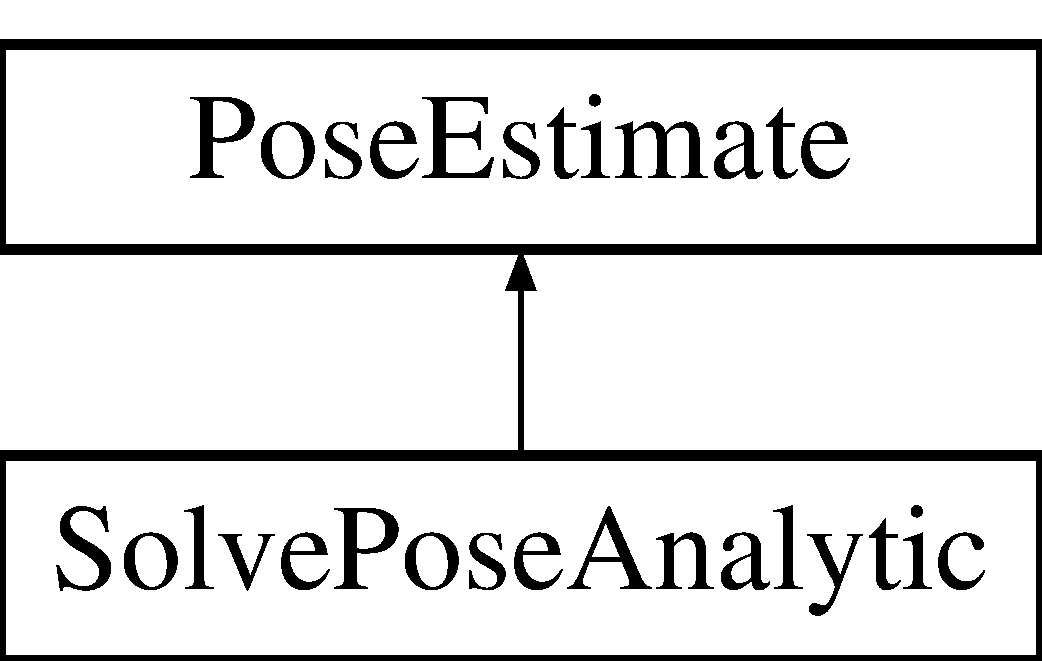
\includegraphics[height=2.000000cm]{classSolvePoseAnalytic}
\end{center}
\end{figure}
\subsection*{\-Public \-Member \-Functions}
\begin{DoxyCompactItemize}
\item 
\hyperlink{classSolvePoseAnalytic_a46909a99ed0f06e70aa4b9d999c6356b}{\-Solve\-Pose\-Analytic} ()
\begin{DoxyCompactList}\small\item\em \-Constructor, sets default parameters. \end{DoxyCompactList}\item 
\hyperlink{classSolvePoseAnalytic_a0bce3ad52a52f23cd14eabd7de12d832}{$\sim$\-Solve\-Pose\-Analytic} ()
\begin{DoxyCompactList}\small\item\em \-Destructor, currently not implemented. \end{DoxyCompactList}\item 
void \hyperlink{classSolvePoseAnalytic_a0a3fd0af007d4a945c03f49f820badcf}{estimate\-Pose} ()
\begin{DoxyCompactList}\small\item\em \-Implementation of the analytic pose estimation algorithm. \end{DoxyCompactList}\item 
void \hyperlink{classSolvePoseAnalytic_aff3d9a1a6c15b4076d8fc560fd18176c}{set\-Decomposition} (int method)
\end{DoxyCompactItemize}
\subsection*{\-Private \-Member \-Functions}
\begin{DoxyCompactItemize}
\item 
void \hyperlink{classSolvePoseAnalytic_a1bd5ff12daa4146f5ce418391cb03c7c}{single\-Solver} ()
\begin{DoxyCompactList}\small\item\em \-Analytic solution to pose estimation when only a single computational unit is active. \end{DoxyCompactList}\item 
void \hyperlink{classSolvePoseAnalytic_aea9b5c0833af7633f80b8879b26b4c99}{multi\-Solvers} ()
\begin{DoxyCompactList}\small\item\em \-Pose estimation with multiple computation units. \end{DoxyCompactList}\item 
void \hyperlink{classSolvePoseAnalytic_afdb3d837111ffdfb4fe5821dc6b6165b}{\-A\-D\-M\-M\-Iter} (\-Eigen\-::\-Matrix4f \&dadj, \-Eigen\-::\-Matrix4f \&\-Zn, \-Eigen\-::\-Matrix4f \&\-Y, \-Eigen\-::\-Matrix4f \&\-Z0, float ainv)
\begin{DoxyCompactList}\small\item\em \-Single local \-A\-D\-M\-M pose estimation step. \end{DoxyCompactList}\item 
void \hyperlink{classSolvePoseAnalytic_a477b3c908bc27e07c80ec117a6cfd8d9}{\-Dual\-Iter} ()
\begin{DoxyCompactList}\small\item\em \-In the future, dual ascent may be implemented as an alternative to \-A\-D\-M\-M. \end{DoxyCompactList}\item 
void \hyperlink{classSolvePoseAnalytic_a51160b660f01b388d8e535b00f54336e}{adjoint} (\-Eigen\-::\-Matrix3f \&\-D, \-Eigen\-::\-Matrix4f \&\-Dadj)
\begin{DoxyCompactList}\small\item\em \-Calculate the adjoint of the mapping between \-S\-O(3) and its four dimensional lift. \end{DoxyCompactList}\item 
void \hyperlink{classSolvePoseAnalytic_a5c756fab3a0a31c6f6c02d0a9a0cf62a}{z2so} (\-Eigen\-::\-Matrix4f \&z, \-Eigen\-::\-Matrix3f \&r)
\begin{DoxyCompactList}\small\item\em \-Transformation from 4\-D representation of \-S\-O(3) convex hull to element in \-S\-O(3). \end{DoxyCompactList}\item 
void \hyperlink{classSolvePoseAnalytic_addd843afaa4ce7e35826f100d46e3699}{proj\-Free\-Spectra} (\-Eigen\-::\-Vector4f \&v)
\begin{DoxyCompactList}\small\item\em \-Projection onto the free spectrahedra. \end{DoxyCompactList}\end{DoxyCompactItemize}
\subsection*{\-Private \-Attributes}
\begin{DoxyCompactItemize}
\item 
int \hyperlink{classSolvePoseAnalytic_ae2c640a9416555bb83e8ffbc39e48a0c}{decomp\-\_\-method}
\end{DoxyCompactItemize}


\subsection{\-Detailed \-Description}
\-Pose estimation using analytic solutions to optimization problems over the convex hull of \-S\-O(3). 

\-Unfortunately, analytic solutions are only available for the point to point metric and in the absence of outlier rejection.

\-Parallelization is achieved by splitting the data over a number of cores and using \-A\-D\-M\-M to achieve consensus over the different computation units.

\begin{DoxyAuthor}{\-Author}
\-Matanya \-Horowitz 
\end{DoxyAuthor}
\begin{DoxyDate}{\-Date}
\-July 28, 2014 
\end{DoxyDate}


\subsection{\-Constructor \& \-Destructor \-Documentation}
\hypertarget{classSolvePoseAnalytic_a46909a99ed0f06e70aa4b9d999c6356b}{\index{\-Solve\-Pose\-Analytic@{\-Solve\-Pose\-Analytic}!\-Solve\-Pose\-Analytic@{\-Solve\-Pose\-Analytic}}
\index{\-Solve\-Pose\-Analytic@{\-Solve\-Pose\-Analytic}!SolvePoseAnalytic@{\-Solve\-Pose\-Analytic}}
\subsubsection[{\-Solve\-Pose\-Analytic}]{\setlength{\rightskip}{0pt plus 5cm}{\bf \-Solve\-Pose\-Analytic\-::\-Solve\-Pose\-Analytic} (
\begin{DoxyParamCaption}
{}
\end{DoxyParamCaption}
)}}\label{classSolvePoseAnalytic_a46909a99ed0f06e70aa4b9d999c6356b}


\-Constructor, sets default parameters. 

\hypertarget{classSolvePoseAnalytic_a0bce3ad52a52f23cd14eabd7de12d832}{\index{\-Solve\-Pose\-Analytic@{\-Solve\-Pose\-Analytic}!$\sim$\-Solve\-Pose\-Analytic@{$\sim$\-Solve\-Pose\-Analytic}}
\index{$\sim$\-Solve\-Pose\-Analytic@{$\sim$\-Solve\-Pose\-Analytic}!SolvePoseAnalytic@{\-Solve\-Pose\-Analytic}}
\subsubsection[{$\sim$\-Solve\-Pose\-Analytic}]{\setlength{\rightskip}{0pt plus 5cm}{\bf \-Solve\-Pose\-Analytic\-::$\sim$\-Solve\-Pose\-Analytic} (
\begin{DoxyParamCaption}
{}
\end{DoxyParamCaption}
)}}\label{classSolvePoseAnalytic_a0bce3ad52a52f23cd14eabd7de12d832}


\-Destructor, currently not implemented. 

\mbox{[}\-Todo\mbox{]}\-: \-Memory leaks are possible. 

\subsection{\-Member \-Function \-Documentation}
\hypertarget{classSolvePoseAnalytic_a51160b660f01b388d8e535b00f54336e}{\index{\-Solve\-Pose\-Analytic@{\-Solve\-Pose\-Analytic}!adjoint@{adjoint}}
\index{adjoint@{adjoint}!SolvePoseAnalytic@{\-Solve\-Pose\-Analytic}}
\subsubsection[{adjoint}]{\setlength{\rightskip}{0pt plus 5cm}void {\bf \-Solve\-Pose\-Analytic\-::adjoint} (
\begin{DoxyParamCaption}
\item[{\-Eigen\-::\-Matrix3f \&}]{\-D, }
\item[{\-Eigen\-::\-Matrix4f \&}]{\-Dadj}
\end{DoxyParamCaption}
)\hspace{0.3cm}{\ttfamily  \mbox{[}private\mbox{]}}}}\label{classSolvePoseAnalytic_a51160b660f01b388d8e535b00f54336e}


\-Calculate the adjoint of the mapping between \-S\-O(3) and its four dimensional lift. 


\begin{DoxyParams}[1]{\-Parameters}
\mbox{\tt in}  & {\em \-D} & \-Data matrix to be adjointed. \\
\hline
\mbox{\tt out}  & {\em \-Dadj} & \-The adjoint of the data matrix. \\
\hline
\end{DoxyParams}
\hypertarget{classSolvePoseAnalytic_afdb3d837111ffdfb4fe5821dc6b6165b}{\index{\-Solve\-Pose\-Analytic@{\-Solve\-Pose\-Analytic}!\-A\-D\-M\-M\-Iter@{\-A\-D\-M\-M\-Iter}}
\index{\-A\-D\-M\-M\-Iter@{\-A\-D\-M\-M\-Iter}!SolvePoseAnalytic@{\-Solve\-Pose\-Analytic}}
\subsubsection[{\-A\-D\-M\-M\-Iter}]{\setlength{\rightskip}{0pt plus 5cm}void {\bf \-Solve\-Pose\-Analytic\-::\-A\-D\-M\-M\-Iter} (
\begin{DoxyParamCaption}
\item[{\-Eigen\-::\-Matrix4f \&}]{dadj, }
\item[{\-Eigen\-::\-Matrix4f \&}]{\-Zn, }
\item[{\-Eigen\-::\-Matrix4f \&}]{\-Y, }
\item[{\-Eigen\-::\-Matrix4f \&}]{\-Z0, }
\item[{float}]{ainv}
\end{DoxyParamCaption}
)\hspace{0.3cm}{\ttfamily  \mbox{[}private\mbox{]}}}}\label{classSolvePoseAnalytic_afdb3d837111ffdfb4fe5821dc6b6165b}


\-Single local \-A\-D\-M\-M pose estimation step. 

\mbox{[}\-Todo\mbox{]} \-Make inline for speed.


\begin{DoxyParams}[1]{\-Parameters}
\mbox{\tt in}  & {\em dadj} & \-The adjoint of the local data matrix \\
\hline
\mbox{\tt out}  & {\em \-Zn} & \-The local \-Z optimization variable \\
\hline
\mbox{\tt in}  & {\em \-Y} & \-The local dual price variable \\
\hline
\mbox{\tt in}  & {\em \-Z0} & \-Centralized fusion variable \\
\hline
\mbox{\tt in}  & {\em ainv} & \-The inverse of the \-A\-D\-M\-M gradient variable. \\
\hline
\end{DoxyParams}
\hypertarget{classSolvePoseAnalytic_a477b3c908bc27e07c80ec117a6cfd8d9}{\index{\-Solve\-Pose\-Analytic@{\-Solve\-Pose\-Analytic}!\-Dual\-Iter@{\-Dual\-Iter}}
\index{\-Dual\-Iter@{\-Dual\-Iter}!SolvePoseAnalytic@{\-Solve\-Pose\-Analytic}}
\subsubsection[{\-Dual\-Iter}]{\setlength{\rightskip}{0pt plus 5cm}void {\bf \-Solve\-Pose\-Analytic\-::\-Dual\-Iter} (
\begin{DoxyParamCaption}
{}
\end{DoxyParamCaption}
)\hspace{0.3cm}{\ttfamily  \mbox{[}private\mbox{]}}}}\label{classSolvePoseAnalytic_a477b3c908bc27e07c80ec117a6cfd8d9}


\-In the future, dual ascent may be implemented as an alternative to \-A\-D\-M\-M. 

\hypertarget{classSolvePoseAnalytic_a0a3fd0af007d4a945c03f49f820badcf}{\index{\-Solve\-Pose\-Analytic@{\-Solve\-Pose\-Analytic}!estimate\-Pose@{estimate\-Pose}}
\index{estimate\-Pose@{estimate\-Pose}!SolvePoseAnalytic@{\-Solve\-Pose\-Analytic}}
\subsubsection[{estimate\-Pose}]{\setlength{\rightskip}{0pt plus 5cm}void {\bf \-Solve\-Pose\-Analytic\-::estimate\-Pose} (
\begin{DoxyParamCaption}
{}
\end{DoxyParamCaption}
)\hspace{0.3cm}{\ttfamily  \mbox{[}virtual\mbox{]}}}}\label{classSolvePoseAnalytic_a0a3fd0af007d4a945c03f49f820badcf}


\-Implementation of the analytic pose estimation algorithm. 



\-Implements \hyperlink{classPoseEstimate_a6fdf8eec3cadac69bcf8181c89d82903}{\-Pose\-Estimate}.

\hypertarget{classSolvePoseAnalytic_aea9b5c0833af7633f80b8879b26b4c99}{\index{\-Solve\-Pose\-Analytic@{\-Solve\-Pose\-Analytic}!multi\-Solvers@{multi\-Solvers}}
\index{multi\-Solvers@{multi\-Solvers}!SolvePoseAnalytic@{\-Solve\-Pose\-Analytic}}
\subsubsection[{multi\-Solvers}]{\setlength{\rightskip}{0pt plus 5cm}void {\bf \-Solve\-Pose\-Analytic\-::multi\-Solvers} (
\begin{DoxyParamCaption}
{}
\end{DoxyParamCaption}
)\hspace{0.3cm}{\ttfamily  \mbox{[}private\mbox{]}}}}\label{classSolvePoseAnalytic_aea9b5c0833af7633f80b8879b26b4c99}


\-Pose estimation with multiple computation units. 

\-Open\-M\-P allows for estimation to be done over subsets of the data. \-At each iteration the local estimates are combined via an \-A\-D\-M\-M update over relaxation parameters. \-See \char`\"{}\-A Convex Approach to Consensus on S\-O(n)\char`\"{} by \-Matni and \-Horowitz for details. \hypertarget{classSolvePoseAnalytic_addd843afaa4ce7e35826f100d46e3699}{\index{\-Solve\-Pose\-Analytic@{\-Solve\-Pose\-Analytic}!proj\-Free\-Spectra@{proj\-Free\-Spectra}}
\index{proj\-Free\-Spectra@{proj\-Free\-Spectra}!SolvePoseAnalytic@{\-Solve\-Pose\-Analytic}}
\subsubsection[{proj\-Free\-Spectra}]{\setlength{\rightskip}{0pt plus 5cm}void {\bf \-Solve\-Pose\-Analytic\-::proj\-Free\-Spectra} (
\begin{DoxyParamCaption}
\item[{\-Eigen\-::\-Vector4f \&}]{v}
\end{DoxyParamCaption}
)\hspace{0.3cm}{\ttfamily  \mbox{[}private\mbox{]}}}}\label{classSolvePoseAnalytic_addd843afaa4ce7e35826f100d46e3699}


\-Projection onto the free spectrahedra. 


\begin{DoxyParams}[1]{\-Parameters}
\mbox{\tt in,out}  & {\em v} & \-Vector to be projected. \-Overwritten with the result. \\
\hline
\end{DoxyParams}
\hypertarget{classSolvePoseAnalytic_aff3d9a1a6c15b4076d8fc560fd18176c}{\index{\-Solve\-Pose\-Analytic@{\-Solve\-Pose\-Analytic}!set\-Decomposition@{set\-Decomposition}}
\index{set\-Decomposition@{set\-Decomposition}!SolvePoseAnalytic@{\-Solve\-Pose\-Analytic}}
\subsubsection[{set\-Decomposition}]{\setlength{\rightskip}{0pt plus 5cm}void {\bf \-Solve\-Pose\-Analytic\-::set\-Decomposition} (
\begin{DoxyParamCaption}
\item[{int}]{method}
\end{DoxyParamCaption}
)}}\label{classSolvePoseAnalytic_aff3d9a1a6c15b4076d8fc560fd18176c}
\hypertarget{classSolvePoseAnalytic_a1bd5ff12daa4146f5ce418391cb03c7c}{\index{\-Solve\-Pose\-Analytic@{\-Solve\-Pose\-Analytic}!single\-Solver@{single\-Solver}}
\index{single\-Solver@{single\-Solver}!SolvePoseAnalytic@{\-Solve\-Pose\-Analytic}}
\subsubsection[{single\-Solver}]{\setlength{\rightskip}{0pt plus 5cm}void {\bf \-Solve\-Pose\-Analytic\-::single\-Solver} (
\begin{DoxyParamCaption}
{}
\end{DoxyParamCaption}
)\hspace{0.3cm}{\ttfamily  \mbox{[}private\mbox{]}}}}\label{classSolvePoseAnalytic_a1bd5ff12daa4146f5ce418391cb03c7c}


\-Analytic solution to pose estimation when only a single computational unit is active. 

\begin{DoxySeeAlso}{\-See also}
\hyperlink{classSolvePoseAnalytic_aea9b5c0833af7633f80b8879b26b4c99}{multi\-Solvers()} 
\end{DoxySeeAlso}
\hypertarget{classSolvePoseAnalytic_a5c756fab3a0a31c6f6c02d0a9a0cf62a}{\index{\-Solve\-Pose\-Analytic@{\-Solve\-Pose\-Analytic}!z2so@{z2so}}
\index{z2so@{z2so}!SolvePoseAnalytic@{\-Solve\-Pose\-Analytic}}
\subsubsection[{z2so}]{\setlength{\rightskip}{0pt plus 5cm}void {\bf \-Solve\-Pose\-Analytic\-::z2so} (
\begin{DoxyParamCaption}
\item[{\-Eigen\-::\-Matrix4f \&}]{z, }
\item[{\-Eigen\-::\-Matrix3f \&}]{r}
\end{DoxyParamCaption}
)\hspace{0.3cm}{\ttfamily  \mbox{[}private\mbox{]}}}}\label{classSolvePoseAnalytic_a5c756fab3a0a31c6f6c02d0a9a0cf62a}


\-Transformation from 4\-D representation of \-S\-O(3) convex hull to element in \-S\-O(3). 


\begin{DoxyParams}[1]{\-Parameters}
\mbox{\tt in}  & {\em z} & \-Object in lifted co\mbox{[}\-S\-O(3)\mbox{]} representation. \\
\hline
\mbox{\tt out}  & {\em r} & \-Element in co(\-S\-O) \\
\hline
\end{DoxyParams}


\subsection{\-Member \-Data \-Documentation}
\hypertarget{classSolvePoseAnalytic_ae2c640a9416555bb83e8ffbc39e48a0c}{\index{\-Solve\-Pose\-Analytic@{\-Solve\-Pose\-Analytic}!decomp\-\_\-method@{decomp\-\_\-method}}
\index{decomp\-\_\-method@{decomp\-\_\-method}!SolvePoseAnalytic@{\-Solve\-Pose\-Analytic}}
\subsubsection[{decomp\-\_\-method}]{\setlength{\rightskip}{0pt plus 5cm}int {\bf \-Solve\-Pose\-Analytic\-::decomp\-\_\-method}\hspace{0.3cm}{\ttfamily  \mbox{[}private\mbox{]}}}}\label{classSolvePoseAnalytic_ae2c640a9416555bb83e8ffbc39e48a0c}


\-The documentation for this class was generated from the following files\-:\begin{DoxyCompactItemize}
\item 
\-Cvx\-\_\-\-Pose/src/\hyperlink{SolvePoseAnalytic_8h}{\-Solve\-Pose\-Analytic.\-h}\item 
\-Cvx\-\_\-\-Pose/src/\hyperlink{SolvePoseAnalytic_8cpp}{\-Solve\-Pose\-Analytic.\-cpp}\end{DoxyCompactItemize}

\hypertarget{classSolvePoseCVX}{\section{\-Solve\-Pose\-C\-V\-X \-Class \-Reference}
\label{classSolvePoseCVX}\index{\-Solve\-Pose\-C\-V\-X@{\-Solve\-Pose\-C\-V\-X}}
}


\-Pose estimation using the convex hull of \-S\-O(3) via a semidefinite program.  




{\ttfamily \#include $<$\-Solve\-Pose\-C\-V\-X.\-h$>$}

\-Inheritance diagram for \-Solve\-Pose\-C\-V\-X\-:\begin{figure}[H]
\begin{center}
\leavevmode
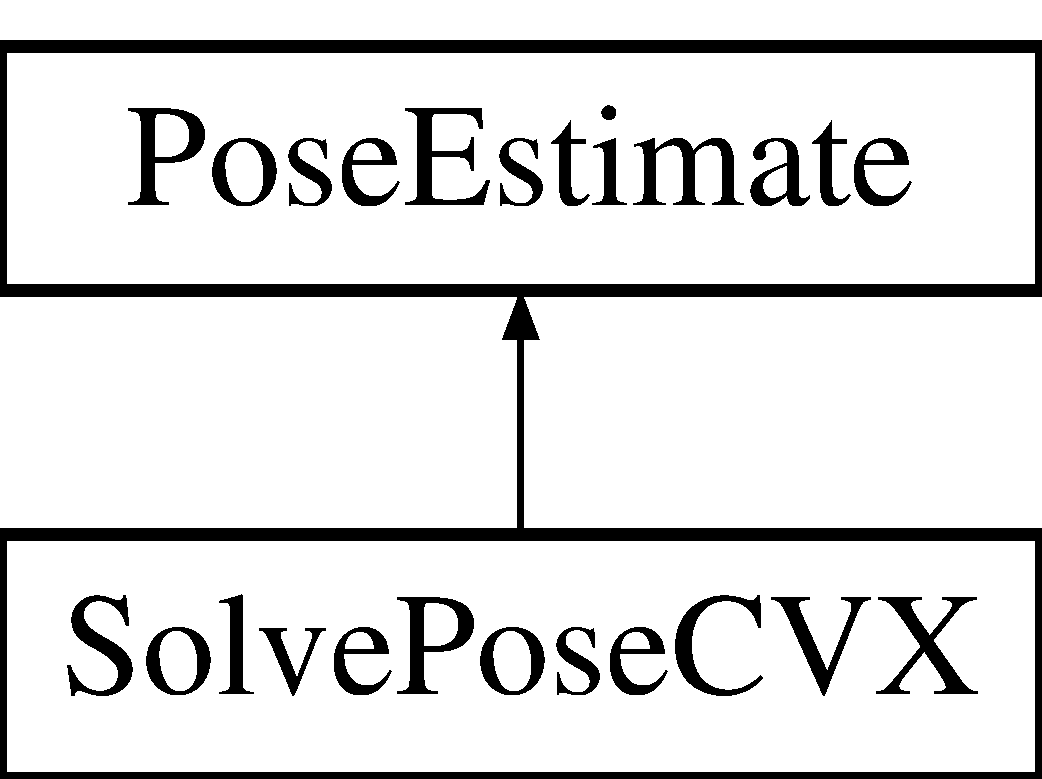
\includegraphics[height=2.000000cm]{classSolvePoseCVX}
\end{center}
\end{figure}
\subsection*{\-Public \-Member \-Functions}
\begin{DoxyCompactItemize}
\item 
\hyperlink{classSolvePoseCVX_a482baaffc4162260c7e565b1fa623007}{\-Solve\-Pose\-C\-V\-X} ()
\begin{DoxyCompactList}\small\item\em \-Constructor, which sets default solution parameters. \end{DoxyCompactList}\item 
\hyperlink{classSolvePoseCVX_a00a0ef0e4c0c55bde6d63c03c496082d}{$\sim$\-Solve\-Pose\-C\-V\-X} ()
\begin{DoxyCompactList}\small\item\em \-Destructor, which isn't currently implemented. \end{DoxyCompactList}\item 
void \hyperlink{classSolvePoseCVX_a081c857ff6c1c9e6597d41fb08bb6f16}{estimate\-Pose} ()
\begin{DoxyCompactList}\small\item\em \-Performs the pose estimation using an \-S\-D\-P. \end{DoxyCompactList}\item 
void \hyperlink{classSolvePoseCVX_a413870a9249a7f3b2ceb0ba52f68cb5f}{set\-Decomposition} (int method)
\begin{DoxyCompactList}\small\item\em \-Set the decomposition. \end{DoxyCompactList}\end{DoxyCompactItemize}
\subsection*{\-Private \-Member \-Functions}
\begin{DoxyCompactItemize}
\item 
void \hyperlink{classSolvePoseCVX_ac6c5c12f31943c02eac2b4e3afe95cb5}{single\-Solver} ()
\begin{DoxyCompactList}\small\item\em \-Solve the \-S\-D\-P with only a single computation element. \end{DoxyCompactList}\item 
void \hyperlink{classSolvePoseCVX_aa15afe19bca14542c1466f4582a8408a}{multi\-Solvers} ()
\begin{DoxyCompactList}\small\item\em \-Unimplemented \mbox{[}\-Todo\mbox{]} parallelization of the \-S\-D\-P using \-A\-D\-M\-M and \-Open\-M\-P. \end{DoxyCompactList}\item 
void \hyperlink{classSolvePoseCVX_af71375a8ebc356e5794249ae0c1243d6}{initialize\-Solver} ()
\begin{DoxyCompactList}\small\item\em \-Initialize the convex solver and parameters. \end{DoxyCompactList}\item 
void \hyperlink{classSolvePoseCVX_aadfc695ad82f44103e7e51c037ddb232}{init\-S\-D\-P\-A\-Cons\-Matrix} (int k, int l)
\begin{DoxyCompactList}\small\item\em \-Utility function to encode the \-A\-\_\-\{i,j\} constraints. \end{DoxyCompactList}\item 
void \hyperlink{classSolvePoseCVX_ac1b83848a5b98e008dfc9b7a87b0079c}{setup\-Quadratic\-Objective} ()
\begin{DoxyCompactList}\small\item\em \-Sets up the optimization with a quadratic objective. \end{DoxyCompactList}\item 
void \hyperlink{classSolvePoseCVX_a4e1c078bdb3a613349c7136bdb0899b9}{setup\-R\-Constraint} ()
\begin{DoxyCompactList}\small\item\em \-Sets up the \-C\-O(\-S\-O(3)) constraint. \end{DoxyCompactList}\item 
void \hyperlink{classSolvePoseCVX_adba2454a08d9e6115cd075928c1d5518}{setup\-Linear\-Objective} ()
\begin{DoxyCompactList}\small\item\em \-Sets up the linear objective. \end{DoxyCompactList}\end{DoxyCompactItemize}
\subsection*{\-Private \-Attributes}
\begin{DoxyCompactItemize}
\item 
int \hyperlink{classSolvePoseCVX_a6d4be163f9b06fc013c99bbacceece14}{decomp\-\_\-method}
\item 
\-S\-D\-P\-A \hyperlink{classSolvePoseCVX_af0c222b2ce7361ff8a54eee918ea1c65}{sdpa}
\begin{DoxyCompactList}\small\item\em \-S\-D\-P\-A interface for numerically solving the convex problem. \end{DoxyCompactList}\end{DoxyCompactItemize}


\subsection{\-Detailed \-Description}
\-Pose estimation using the convex hull of \-S\-O(3) via a semidefinite program. 

\-The semidefinite formulation allows us to include the point to plane metric as well as outlier rejection using a \-L\-A\-S\-S\-O penalty. \-Currently, the publicly available \-S\-D\-P\-A package is used as our semidefinite solver.

\begin{DoxyAuthor}{\-Author}
\-Matanya \-Horowitz 
\end{DoxyAuthor}
\begin{DoxyDate}{\-Date}
\-July 28 2014 
\end{DoxyDate}


\subsection{\-Constructor \& \-Destructor \-Documentation}
\hypertarget{classSolvePoseCVX_a482baaffc4162260c7e565b1fa623007}{\index{\-Solve\-Pose\-C\-V\-X@{\-Solve\-Pose\-C\-V\-X}!\-Solve\-Pose\-C\-V\-X@{\-Solve\-Pose\-C\-V\-X}}
\index{\-Solve\-Pose\-C\-V\-X@{\-Solve\-Pose\-C\-V\-X}!SolvePoseCVX@{\-Solve\-Pose\-C\-V\-X}}
\subsubsection[{\-Solve\-Pose\-C\-V\-X}]{\setlength{\rightskip}{0pt plus 5cm}{\bf \-Solve\-Pose\-C\-V\-X\-::\-Solve\-Pose\-C\-V\-X} (
\begin{DoxyParamCaption}
{}
\end{DoxyParamCaption}
)}}\label{classSolvePoseCVX_a482baaffc4162260c7e565b1fa623007}


\-Constructor, which sets default solution parameters. 

\hypertarget{classSolvePoseCVX_a00a0ef0e4c0c55bde6d63c03c496082d}{\index{\-Solve\-Pose\-C\-V\-X@{\-Solve\-Pose\-C\-V\-X}!$\sim$\-Solve\-Pose\-C\-V\-X@{$\sim$\-Solve\-Pose\-C\-V\-X}}
\index{$\sim$\-Solve\-Pose\-C\-V\-X@{$\sim$\-Solve\-Pose\-C\-V\-X}!SolvePoseCVX@{\-Solve\-Pose\-C\-V\-X}}
\subsubsection[{$\sim$\-Solve\-Pose\-C\-V\-X}]{\setlength{\rightskip}{0pt plus 5cm}{\bf \-Solve\-Pose\-C\-V\-X\-::$\sim$\-Solve\-Pose\-C\-V\-X} (
\begin{DoxyParamCaption}
{}
\end{DoxyParamCaption}
)}}\label{classSolvePoseCVX_a00a0ef0e4c0c55bde6d63c03c496082d}


\-Destructor, which isn't currently implemented. 

\mbox{[}\-Todo\mbox{]} \-There may be memory leaks. 

\subsection{\-Member \-Function \-Documentation}
\hypertarget{classSolvePoseCVX_a081c857ff6c1c9e6597d41fb08bb6f16}{\index{\-Solve\-Pose\-C\-V\-X@{\-Solve\-Pose\-C\-V\-X}!estimate\-Pose@{estimate\-Pose}}
\index{estimate\-Pose@{estimate\-Pose}!SolvePoseCVX@{\-Solve\-Pose\-C\-V\-X}}
\subsubsection[{estimate\-Pose}]{\setlength{\rightskip}{0pt plus 5cm}void {\bf \-Solve\-Pose\-C\-V\-X\-::estimate\-Pose} (
\begin{DoxyParamCaption}
{}
\end{DoxyParamCaption}
)\hspace{0.3cm}{\ttfamily  \mbox{[}virtual\mbox{]}}}}\label{classSolvePoseCVX_a081c857ff6c1c9e6597d41fb08bb6f16}


\-Performs the pose estimation using an \-S\-D\-P. 



\-Implements \hyperlink{classPoseEstimate_a6fdf8eec3cadac69bcf8181c89d82903}{\-Pose\-Estimate}.

\hypertarget{classSolvePoseCVX_af71375a8ebc356e5794249ae0c1243d6}{\index{\-Solve\-Pose\-C\-V\-X@{\-Solve\-Pose\-C\-V\-X}!initialize\-Solver@{initialize\-Solver}}
\index{initialize\-Solver@{initialize\-Solver}!SolvePoseCVX@{\-Solve\-Pose\-C\-V\-X}}
\subsubsection[{initialize\-Solver}]{\setlength{\rightskip}{0pt plus 5cm}void {\bf \-Solve\-Pose\-C\-V\-X\-::initialize\-Solver} (
\begin{DoxyParamCaption}
{}
\end{DoxyParamCaption}
)\hspace{0.3cm}{\ttfamily  \mbox{[}private\mbox{]}}}}\label{classSolvePoseCVX_af71375a8ebc356e5794249ae0c1243d6}


\-Initialize the convex solver and parameters. 

\-The presence of outlier rejection requires different initialization (there are many more optimization variables). \hypertarget{classSolvePoseCVX_aadfc695ad82f44103e7e51c037ddb232}{\index{\-Solve\-Pose\-C\-V\-X@{\-Solve\-Pose\-C\-V\-X}!init\-S\-D\-P\-A\-Cons\-Matrix@{init\-S\-D\-P\-A\-Cons\-Matrix}}
\index{init\-S\-D\-P\-A\-Cons\-Matrix@{init\-S\-D\-P\-A\-Cons\-Matrix}!SolvePoseCVX@{\-Solve\-Pose\-C\-V\-X}}
\subsubsection[{init\-S\-D\-P\-A\-Cons\-Matrix}]{\setlength{\rightskip}{0pt plus 5cm}void {\bf \-Solve\-Pose\-C\-V\-X\-::init\-S\-D\-P\-A\-Cons\-Matrix} (
\begin{DoxyParamCaption}
\item[{int}]{k, }
\item[{int}]{l}
\end{DoxyParamCaption}
)\hspace{0.3cm}{\ttfamily  \mbox{[}private\mbox{]}}}}\label{classSolvePoseCVX_aadfc695ad82f44103e7e51c037ddb232}


\-Utility function to encode the \-A\-\_\-\{i,j\} constraints. 

\begin{DoxySeeAlso}{\-See also}
\hyperlink{classSolvePoseCVX_a4e1c078bdb3a613349c7136bdb0899b9}{setup\-R\-Constraint()} 
\end{DoxySeeAlso}
\hypertarget{classSolvePoseCVX_aa15afe19bca14542c1466f4582a8408a}{\index{\-Solve\-Pose\-C\-V\-X@{\-Solve\-Pose\-C\-V\-X}!multi\-Solvers@{multi\-Solvers}}
\index{multi\-Solvers@{multi\-Solvers}!SolvePoseCVX@{\-Solve\-Pose\-C\-V\-X}}
\subsubsection[{multi\-Solvers}]{\setlength{\rightskip}{0pt plus 5cm}void {\bf \-Solve\-Pose\-C\-V\-X\-::multi\-Solvers} (
\begin{DoxyParamCaption}
{}
\end{DoxyParamCaption}
)\hspace{0.3cm}{\ttfamily  \mbox{[}private\mbox{]}}}}\label{classSolvePoseCVX_aa15afe19bca14542c1466f4582a8408a}


\-Unimplemented \mbox{[}\-Todo\mbox{]} parallelization of the \-S\-D\-P using \-A\-D\-M\-M and \-Open\-M\-P. 

\hypertarget{classSolvePoseCVX_a413870a9249a7f3b2ceb0ba52f68cb5f}{\index{\-Solve\-Pose\-C\-V\-X@{\-Solve\-Pose\-C\-V\-X}!set\-Decomposition@{set\-Decomposition}}
\index{set\-Decomposition@{set\-Decomposition}!SolvePoseCVX@{\-Solve\-Pose\-C\-V\-X}}
\subsubsection[{set\-Decomposition}]{\setlength{\rightskip}{0pt plus 5cm}void {\bf \-Solve\-Pose\-C\-V\-X\-::set\-Decomposition} (
\begin{DoxyParamCaption}
\item[{int}]{method}
\end{DoxyParamCaption}
)}}\label{classSolvePoseCVX_a413870a9249a7f3b2ceb0ba52f68cb5f}


\-Set the decomposition. 

\-I don't remember what this is for \mbox{[}\-Todo\mbox{]}. \hypertarget{classSolvePoseCVX_adba2454a08d9e6115cd075928c1d5518}{\index{\-Solve\-Pose\-C\-V\-X@{\-Solve\-Pose\-C\-V\-X}!setup\-Linear\-Objective@{setup\-Linear\-Objective}}
\index{setup\-Linear\-Objective@{setup\-Linear\-Objective}!SolvePoseCVX@{\-Solve\-Pose\-C\-V\-X}}
\subsubsection[{setup\-Linear\-Objective}]{\setlength{\rightskip}{0pt plus 5cm}void {\bf \-Solve\-Pose\-C\-V\-X\-::setup\-Linear\-Objective} (
\begin{DoxyParamCaption}
{}
\end{DoxyParamCaption}
)\hspace{0.3cm}{\ttfamily  \mbox{[}private\mbox{]}}}}\label{classSolvePoseCVX_adba2454a08d9e6115cd075928c1d5518}


\-Sets up the linear objective. 

\-Note that this objective produces solutions guaranteed to be elements of \-S\-O(3), but does not allow for the point to plane metric or outlier rejection to be incorporated. \hypertarget{classSolvePoseCVX_ac1b83848a5b98e008dfc9b7a87b0079c}{\index{\-Solve\-Pose\-C\-V\-X@{\-Solve\-Pose\-C\-V\-X}!setup\-Quadratic\-Objective@{setup\-Quadratic\-Objective}}
\index{setup\-Quadratic\-Objective@{setup\-Quadratic\-Objective}!SolvePoseCVX@{\-Solve\-Pose\-C\-V\-X}}
\subsubsection[{setup\-Quadratic\-Objective}]{\setlength{\rightskip}{0pt plus 5cm}void {\bf \-Solve\-Pose\-C\-V\-X\-::setup\-Quadratic\-Objective} (
\begin{DoxyParamCaption}
{}
\end{DoxyParamCaption}
)\hspace{0.3cm}{\ttfamily  \mbox{[}private\mbox{]}}}}\label{classSolvePoseCVX_ac1b83848a5b98e008dfc9b7a87b0079c}


\-Sets up the optimization with a quadratic objective. 

\-This is necessary when there is an \-L1 penalty or the point to plane metric is used. \-Note that the quadratic objective does not guarantee the solution will be an element of \-S\-O(3). \hypertarget{classSolvePoseCVX_a4e1c078bdb3a613349c7136bdb0899b9}{\index{\-Solve\-Pose\-C\-V\-X@{\-Solve\-Pose\-C\-V\-X}!setup\-R\-Constraint@{setup\-R\-Constraint}}
\index{setup\-R\-Constraint@{setup\-R\-Constraint}!SolvePoseCVX@{\-Solve\-Pose\-C\-V\-X}}
\subsubsection[{setup\-R\-Constraint}]{\setlength{\rightskip}{0pt plus 5cm}void {\bf \-Solve\-Pose\-C\-V\-X\-::setup\-R\-Constraint} (
\begin{DoxyParamCaption}
{}
\end{DoxyParamCaption}
)\hspace{0.3cm}{\ttfamily  \mbox{[}private\mbox{]}}}}\label{classSolvePoseCVX_a4e1c078bdb3a613349c7136bdb0899b9}


\-Sets up the \-C\-O(\-S\-O(3)) constraint. 

\hypertarget{classSolvePoseCVX_ac6c5c12f31943c02eac2b4e3afe95cb5}{\index{\-Solve\-Pose\-C\-V\-X@{\-Solve\-Pose\-C\-V\-X}!single\-Solver@{single\-Solver}}
\index{single\-Solver@{single\-Solver}!SolvePoseCVX@{\-Solve\-Pose\-C\-V\-X}}
\subsubsection[{single\-Solver}]{\setlength{\rightskip}{0pt plus 5cm}void {\bf \-Solve\-Pose\-C\-V\-X\-::single\-Solver} (
\begin{DoxyParamCaption}
{}
\end{DoxyParamCaption}
)\hspace{0.3cm}{\ttfamily  \mbox{[}private\mbox{]}}}}\label{classSolvePoseCVX_ac6c5c12f31943c02eac2b4e3afe95cb5}


\-Solve the \-S\-D\-P with only a single computation element. 

\mbox{[}\-Todo\mbox{]} \-Initial guesses are currently ignored (no warm start). 

\subsection{\-Member \-Data \-Documentation}
\hypertarget{classSolvePoseCVX_a6d4be163f9b06fc013c99bbacceece14}{\index{\-Solve\-Pose\-C\-V\-X@{\-Solve\-Pose\-C\-V\-X}!decomp\-\_\-method@{decomp\-\_\-method}}
\index{decomp\-\_\-method@{decomp\-\_\-method}!SolvePoseCVX@{\-Solve\-Pose\-C\-V\-X}}
\subsubsection[{decomp\-\_\-method}]{\setlength{\rightskip}{0pt plus 5cm}int {\bf \-Solve\-Pose\-C\-V\-X\-::decomp\-\_\-method}\hspace{0.3cm}{\ttfamily  \mbox{[}private\mbox{]}}}}\label{classSolvePoseCVX_a6d4be163f9b06fc013c99bbacceece14}
\hypertarget{classSolvePoseCVX_af0c222b2ce7361ff8a54eee918ea1c65}{\index{\-Solve\-Pose\-C\-V\-X@{\-Solve\-Pose\-C\-V\-X}!sdpa@{sdpa}}
\index{sdpa@{sdpa}!SolvePoseCVX@{\-Solve\-Pose\-C\-V\-X}}
\subsubsection[{sdpa}]{\setlength{\rightskip}{0pt plus 5cm}\-S\-D\-P\-A {\bf \-Solve\-Pose\-C\-V\-X\-::sdpa}\hspace{0.3cm}{\ttfamily  \mbox{[}private\mbox{]}}}}\label{classSolvePoseCVX_af0c222b2ce7361ff8a54eee918ea1c65}


\-S\-D\-P\-A interface for numerically solving the convex problem. 



\-The documentation for this class was generated from the following files\-:\begin{DoxyCompactItemize}
\item 
\-Cvx\-\_\-\-Pose/src/\hyperlink{SolvePoseCVX_8h}{\-Solve\-Pose\-C\-V\-X.\-h}\item 
\-Cvx\-\_\-\-Pose/src/\hyperlink{SolvePoseCVX_8cpp}{\-Solve\-Pose\-C\-V\-X.\-cpp}\end{DoxyCompactItemize}

\hypertarget{structSolverSettings}{\section{\-Solver\-Settings \-Struct \-Reference}
\label{structSolverSettings}\index{\-Solver\-Settings@{\-Solver\-Settings}}
}


{\ttfamily \#include $<$common.\-h$>$}

\subsection*{\-Public \-Attributes}
\begin{DoxyCompactItemize}
\item 
int \hyperlink{structSolverSettings_acf7de9862fb4276d91a1319f220b564a}{metric}
\item 
bool \hyperlink{structSolverSettings_a82eb7bb6b04a2ce6588f8dec8ba09ae5}{outlier\-Rejection}
\item 
float \hyperlink{structSolverSettings_af42a46e051dd69c1bf2f2aa208a8be8f}{tolerance}
\item 
int \hyperlink{structSolverSettings_a6c340bb77bf658db01c727c5e847ddf9}{cores}
\item 
int \hyperlink{structSolverSettings_abd3876067bab2a3808e4c43586a97ff0}{parallel\-Solvers}
\item 
int \hyperlink{structSolverSettings_a83783c865ae94804cf034840547f6d56}{options}
\end{DoxyCompactItemize}


\subsection{\-Member \-Data \-Documentation}
\hypertarget{structSolverSettings_a6c340bb77bf658db01c727c5e847ddf9}{\index{\-Solver\-Settings@{\-Solver\-Settings}!cores@{cores}}
\index{cores@{cores}!SolverSettings@{\-Solver\-Settings}}
\subsubsection[{cores}]{\setlength{\rightskip}{0pt plus 5cm}int {\bf \-Solver\-Settings\-::cores}}}\label{structSolverSettings_a6c340bb77bf658db01c727c5e847ddf9}
\hypertarget{structSolverSettings_acf7de9862fb4276d91a1319f220b564a}{\index{\-Solver\-Settings@{\-Solver\-Settings}!metric@{metric}}
\index{metric@{metric}!SolverSettings@{\-Solver\-Settings}}
\subsubsection[{metric}]{\setlength{\rightskip}{0pt plus 5cm}int {\bf \-Solver\-Settings\-::metric}}}\label{structSolverSettings_acf7de9862fb4276d91a1319f220b564a}
\hypertarget{structSolverSettings_a83783c865ae94804cf034840547f6d56}{\index{\-Solver\-Settings@{\-Solver\-Settings}!options@{options}}
\index{options@{options}!SolverSettings@{\-Solver\-Settings}}
\subsubsection[{options}]{\setlength{\rightskip}{0pt plus 5cm}int {\bf \-Solver\-Settings\-::options}}}\label{structSolverSettings_a83783c865ae94804cf034840547f6d56}
\hypertarget{structSolverSettings_a82eb7bb6b04a2ce6588f8dec8ba09ae5}{\index{\-Solver\-Settings@{\-Solver\-Settings}!outlier\-Rejection@{outlier\-Rejection}}
\index{outlier\-Rejection@{outlier\-Rejection}!SolverSettings@{\-Solver\-Settings}}
\subsubsection[{outlier\-Rejection}]{\setlength{\rightskip}{0pt plus 5cm}bool {\bf \-Solver\-Settings\-::outlier\-Rejection}}}\label{structSolverSettings_a82eb7bb6b04a2ce6588f8dec8ba09ae5}
\hypertarget{structSolverSettings_abd3876067bab2a3808e4c43586a97ff0}{\index{\-Solver\-Settings@{\-Solver\-Settings}!parallel\-Solvers@{parallel\-Solvers}}
\index{parallel\-Solvers@{parallel\-Solvers}!SolverSettings@{\-Solver\-Settings}}
\subsubsection[{parallel\-Solvers}]{\setlength{\rightskip}{0pt plus 5cm}int {\bf \-Solver\-Settings\-::parallel\-Solvers}}}\label{structSolverSettings_abd3876067bab2a3808e4c43586a97ff0}
\hypertarget{structSolverSettings_af42a46e051dd69c1bf2f2aa208a8be8f}{\index{\-Solver\-Settings@{\-Solver\-Settings}!tolerance@{tolerance}}
\index{tolerance@{tolerance}!SolverSettings@{\-Solver\-Settings}}
\subsubsection[{tolerance}]{\setlength{\rightskip}{0pt plus 5cm}float {\bf \-Solver\-Settings\-::tolerance}}}\label{structSolverSettings_af42a46e051dd69c1bf2f2aa208a8be8f}


\-The documentation for this struct was generated from the following file\-:\begin{DoxyCompactItemize}
\item 
\-Cvx\-\_\-\-Pose/src/\hyperlink{common_8h}{common.\-h}\end{DoxyCompactItemize}

\chapter{\-File \-Documentation}
\hypertarget{bunny_8cpp}{\section{\-Cvx\-\_\-\-Pose/examples/bunny.cpp \-File \-Reference}
\label{bunny_8cpp}\index{\-Cvx\-\_\-\-Pose/examples/bunny.\-cpp@{\-Cvx\-\_\-\-Pose/examples/bunny.\-cpp}}
}
{\ttfamily \#include \char`\"{}../src/common.\-h\char`\"{}}\*
{\ttfamily \#include \char`\"{}../src/\-I\-C\-P.\-h\char`\"{}}\*
{\ttfamily \#include $<$iostream$>$}\*
{\ttfamily \#include $<$fstream$>$}\*
{\ttfamily \#include $<$sstream$>$}\*
\subsection*{\-Functions}
\begin{DoxyCompactItemize}
\item 
int \hyperlink{bunny_8cpp_ae66f6b31b5ad750f1fe042a706a4e3d4}{main} ()
\end{DoxyCompactItemize}


\subsection{\-Function \-Documentation}
\hypertarget{bunny_8cpp_ae66f6b31b5ad750f1fe042a706a4e3d4}{\index{bunny.\-cpp@{bunny.\-cpp}!main@{main}}
\index{main@{main}!bunny.cpp@{bunny.\-cpp}}
\subsubsection[{main}]{\setlength{\rightskip}{0pt plus 5cm}int {\bf main} (
\begin{DoxyParamCaption}
{}
\end{DoxyParamCaption}
)}}\label{bunny_8cpp_ae66f6b31b5ad750f1fe042a706a4e3d4}

\hypertarget{common_8h}{\section{\-Cvx\-\_\-\-Pose/src/common.h \-File \-Reference}
\label{common_8h}\index{\-Cvx\-\_\-\-Pose/src/common.\-h@{\-Cvx\-\_\-\-Pose/src/common.\-h}}
}
{\ttfamily \#include $<$\-Eigen/\-Dense$>$}\*
{\ttfamily \#include $<$\-Eigen/\-Core$>$}\*
{\ttfamily \#include $<$\-Eigen/\-Sparse\-Core$>$}\*
{\ttfamily \#include $<$\-Eigen/\-Sparse$>$}\*
{\ttfamily \#include \char`\"{}pcl/kdtree/impl/kdtree\-\_\-flann.\-hpp\char`\"{}}\*
{\ttfamily \#include $<$pcl/point\-\_\-cloud.\-h$>$}\*
{\ttfamily \#include $<$pcl/point\-\_\-types.\-h$>$}\*
\subsection*{\-Classes}
\begin{DoxyCompactItemize}
\item 
struct \hyperlink{structSolverSettings}{\-Solver\-Settings}
\end{DoxyCompactItemize}
\subsection*{\-Typedefs}
\begin{DoxyCompactItemize}
\item 
typedef \-Eigen\-::\-Matrix$<$ float, \*
3, \-Eigen\-::\-Dynamic $>$ \hyperlink{common_8h_a4ec92c19d079ab17709ca464cfb8e5bd}{\-D\-Mat}
\item 
typedef pcl\-::\-Point\-X\-Y\-Z \hyperlink{common_8h_abd10555a534258e2739a38c928ef5db1}{\-Point\-T}
\end{DoxyCompactItemize}


\subsection{\-Typedef \-Documentation}
\hypertarget{common_8h_a4ec92c19d079ab17709ca464cfb8e5bd}{\index{common.\-h@{common.\-h}!\-D\-Mat@{\-D\-Mat}}
\index{\-D\-Mat@{\-D\-Mat}!common.h@{common.\-h}}
\subsubsection[{\-D\-Mat}]{\setlength{\rightskip}{0pt plus 5cm}typedef \-Eigen\-::\-Matrix$<$float,3,\-Eigen\-::\-Dynamic$>$ {\bf \-D\-Mat}}}\label{common_8h_a4ec92c19d079ab17709ca464cfb8e5bd}
\hypertarget{common_8h_abd10555a534258e2739a38c928ef5db1}{\index{common.\-h@{common.\-h}!\-Point\-T@{\-Point\-T}}
\index{\-Point\-T@{\-Point\-T}!common.h@{common.\-h}}
\subsubsection[{\-Point\-T}]{\setlength{\rightskip}{0pt plus 5cm}typedef pcl\-::\-Point\-X\-Y\-Z {\bf \-Point\-T}}}\label{common_8h_abd10555a534258e2739a38c928ef5db1}

\hypertarget{ICP_8cpp}{\section{\-Cvx\-\_\-\-Pose/src/\-I\-C\-P.cpp \-File \-Reference}
\label{ICP_8cpp}\index{\-Cvx\-\_\-\-Pose/src/\-I\-C\-P.\-cpp@{\-Cvx\-\_\-\-Pose/src/\-I\-C\-P.\-cpp}}
}
{\ttfamily \#include \char`\"{}\-I\-C\-P.\-h\char`\"{}}\*

\hypertarget{ICP_8h}{\section{\-Cvx\-\_\-\-Pose/src/\-I\-C\-P.h \-File \-Reference}
\label{ICP_8h}\index{\-Cvx\-\_\-\-Pose/src/\-I\-C\-P.\-h@{\-Cvx\-\_\-\-Pose/src/\-I\-C\-P.\-h}}
}
{\ttfamily \#include \char`\"{}common.\-h\char`\"{}}\*
{\ttfamily \#include \char`\"{}\-Pose\-Estimate.\-h\char`\"{}}\*
{\ttfamily \#include \char`\"{}\-Solve\-Pose\-Analytic.\-h\char`\"{}}\*
{\ttfamily \#include $<$iostream$>$}\*
{\ttfamily \#include $<$pcl/registration/correspondence\-\_\-estimation.\-h$>$}\*
{\ttfamily \#include $<$pcl/common/transforms.\-h$>$}\*
{\ttfamily \#include $<$boost/shared\-\_\-ptr.\-hpp$>$}\*
\subsection*{\-Classes}
\begin{DoxyCompactItemize}
\item 
class \hyperlink{classICP}{\-I\-C\-P}
\begin{DoxyCompactList}\small\item\em \-Iterative \-Closest \-Point. \end{DoxyCompactList}\end{DoxyCompactItemize}

\hypertarget{PoseEstimate_8cpp}{\section{\-Cvx\-\_\-\-Pose/src/\-Pose\-Estimate.cpp \-File \-Reference}
\label{PoseEstimate_8cpp}\index{\-Cvx\-\_\-\-Pose/src/\-Pose\-Estimate.\-cpp@{\-Cvx\-\_\-\-Pose/src/\-Pose\-Estimate.\-cpp}}
}
{\ttfamily \#include \char`\"{}\-Pose\-Estimate.\-h\char`\"{}}\*

\hypertarget{PoseEstimate_8h}{\section{\-Cvx\-\_\-\-Pose/src/\-Pose\-Estimate.h \-File \-Reference}
\label{PoseEstimate_8h}\index{\-Cvx\-\_\-\-Pose/src/\-Pose\-Estimate.\-h@{\-Cvx\-\_\-\-Pose/src/\-Pose\-Estimate.\-h}}
}
{\ttfamily \#include \char`\"{}common.\-h\char`\"{}}\*
{\ttfamily \#include $<$iostream$>$}\*
\subsection*{\-Classes}
\begin{DoxyCompactItemize}
\item 
class \hyperlink{classPoseEstimate}{\-Pose\-Estimate}
\end{DoxyCompactItemize}

\hypertarget{SolvePoseAnalytic_8cpp}{\section{\-Cvx\-\_\-\-Pose/src/\-Solve\-Pose\-Analytic.cpp \-File \-Reference}
\label{SolvePoseAnalytic_8cpp}\index{\-Cvx\-\_\-\-Pose/src/\-Solve\-Pose\-Analytic.\-cpp@{\-Cvx\-\_\-\-Pose/src/\-Solve\-Pose\-Analytic.\-cpp}}
}
{\ttfamily \#include \char`\"{}\-Solve\-Pose\-Analytic.\-h\char`\"{}}\*
{\ttfamily \#include $<$iostream$>$}\*

\hypertarget{SolvePoseAnalytic_8h}{\section{\-Cvx\-\_\-\-Pose/src/\-Solve\-Pose\-Analytic.h \-File \-Reference}
\label{SolvePoseAnalytic_8h}\index{\-Cvx\-\_\-\-Pose/src/\-Solve\-Pose\-Analytic.\-h@{\-Cvx\-\_\-\-Pose/src/\-Solve\-Pose\-Analytic.\-h}}
}
{\ttfamily \#include \char`\"{}common.\-h\char`\"{}}\*
{\ttfamily \#include \char`\"{}\-Pose\-Estimate.\-h\char`\"{}}\*
{\ttfamily \#include $<$iostream$>$}\*
{\ttfamily \#include $<$omp.\-h$>$}\*
\subsection*{\-Classes}
\begin{DoxyCompactItemize}
\item 
class \hyperlink{classSolvePoseAnalytic}{\-Solve\-Pose\-Analytic}
\end{DoxyCompactItemize}

\hypertarget{SolvePoseCVX_8cpp}{\section{\-Cvx\-\_\-\-Pose/src/\-Solve\-Pose\-C\-V\-X.cpp \-File \-Reference}
\label{SolvePoseCVX_8cpp}\index{\-Cvx\-\_\-\-Pose/src/\-Solve\-Pose\-C\-V\-X.\-cpp@{\-Cvx\-\_\-\-Pose/src/\-Solve\-Pose\-C\-V\-X.\-cpp}}
}
{\ttfamily \#include \char`\"{}\-Solve\-Pose\-C\-V\-X.\-h\char`\"{}}\*
{\ttfamily \#include $<$cstdio$>$}\*
{\ttfamily \#include $<$cstdlib$>$}\*

\hypertarget{SolvePoseCVX_8h}{\section{\-Cvx\-\_\-\-Pose/src/\-Solve\-Pose\-C\-V\-X.h \-File \-Reference}
\label{SolvePoseCVX_8h}\index{\-Cvx\-\_\-\-Pose/src/\-Solve\-Pose\-C\-V\-X.\-h@{\-Cvx\-\_\-\-Pose/src/\-Solve\-Pose\-C\-V\-X.\-h}}
}
{\ttfamily \#include $<$iostream$>$}\*
{\ttfamily \#include \char`\"{}\-Pose\-Estimate.\-h\char`\"{}}\*
{\ttfamily \#include \char`\"{}common.\-h\char`\"{}}\*
{\ttfamily \#include $<$sdpa\-\_\-call.\-h$>$}\*
\subsection*{\-Classes}
\begin{DoxyCompactItemize}
\item 
class \hyperlink{classSolvePoseCVX}{\-Solve\-Pose\-C\-V\-X}
\begin{DoxyCompactList}\small\item\em \-Pose estimation using the convex hull of \-S\-O(3) via a semidefinite program. \end{DoxyCompactList}\end{DoxyCompactItemize}

\printindex
\end{document}
